\documentclass[10pt,a4paper]{article}

\usepackage[T1]{fontenc}
\usepackage[utf8]{inputenc}
\usepackage{lmodern}
\usepackage{microtype}
\usepackage[spanish,es-noshorthands]{babel}
\usepackage[table]{xcolor}
\usepackage{booktabs,array,longtable,tabularx,graphicx}
\usepackage{amsmath,amssymb,bm}
\usepackage{siunitx}
\usepackage{tikz}
\usetikzlibrary{arrows.meta,positioning,calc,shapes.geometric}
\usepackage[margin=2cm]{geometry}
\usepackage{fancyhdr}
\usepackage{float}
\usepackage{tcolorbox}
\usepackage{pdflscape}
\usepackage{caption}
\usepackage{enumitem}
\usepackage[colorlinks=true,linkcolor=blue!50!black,urlcolor=blue!50!black]{hyperref}

\sisetup{output-decimal-marker={,}}
\captionsetup{font=small,labelfont=bf}
\setlist{itemsep=2pt,topsep=3pt}
\setlength{\parindent}{0pt}
\setlength{\parskip}{4pt}
\setlength{\headheight}{14pt}
\emergencystretch=2em

\definecolor{ucbblue}{RGB}{0,51,102}
\newcommand{\ep}{e_p}
\newcommand{\eR}{e_R}
\urlstyle{tt}
\newcommand{\ruta}[1]{\path{#1}}
\newcommand{\pend}{\textit{pendiente}}

\pagestyle{fancy}
\fancyhf{}
\lhead{\textbf{IMT-342} \textperiodcentered\ Informe técnico del Hito 3 (ECI-3/4)}
\rhead{ABB IRB~120 + ROS~2}
\cfoot{\thepage}
\renewcommand{\headrulewidth}{0.4pt}

\begin{document}

% ---------------------------------------------------------------- Portada
\begin{center}
{\LARGE\bfseries\color{ucbblue} Validación cinemática, procedencia e integración\\[2pt] ROS--ABB IRB~120\par}
\vspace{4pt}
{\large Informe técnico del Hito 3 (ECI-3/4)\par}
\vspace{6pt}
IMT-342 Robótica \textperiodcentered\ Universidad Católica Boliviana \textperiodcentered\ 2-2026\\
Equipo (según el \texttt{README.md} del proyecto): Dayana Andrade, Mirko Ayala y Marcelo Navarro\\
Versión del documento: borrador del 24/11/2026
\end{center}

\begin{tcolorbox}[colback=yellow!8,colframe=orange!70!black,boxrule=0.6pt,left=3pt,right=3pt,top=2pt,bottom=2pt]
\small\textbf{Estado de este informe.} Es un borrador técnico para revisión del equipo y del docente. No lleva firmas ni autorizaciones: la firma P7 (sección~\ref{sec:p7}), el registro GO/NO-GO de las sesiones de laboratorio y la aprobación de umbrales por el docente figuran como \pend. Todo dato proviene de los archivos del repositorio; lo que no consta se declara como no verificado. Los resultados de FK/IK/$J$ corresponden al paquete \ruta{hito3/validacion}, ejecutado el 24/11/2026 (commit base \texttt{6e82c45}, carpeta \texttt{hito3/} sin versionar en ese momento).
\end{tcolorbox}
\setcounter{tocdepth}{1}
\tableofcontents

% ---------------------------------------------------------------- 1
\section{Resumen y alcance}
\label{sec:resumen}

El informe documenta la validación de los modelos cinemáticos propios del IRB~120 (FK, IK y Jacobiano), la procedencia de los datos usados, la cadena de integración PC$\to$IRC5 y el nivel de evidencia que sostiene cada afirmación. Se sigue la estructura de los criterios unificados de la sesión W14-S02 (Bloques B a H, plantillas P1 a P7) y la rúbrica del ECI-3/4.

\subsection{Niveles de evidencia usados}
Se usa la escala oficial S0--S3: \textbf{S0} modelo o simulación offline; \textbf{S1} observación del controlador con interfaz, unidad, fuente y marca temporal; \textbf{S2} observación trazada en ROS; \textbf{S3} ejecución física autorizada (orden verificable $\to$ aceptación $\to$ estado $\to$ movimiento observado, con registros).

\begin{table}[H]
\centering\small
\renewcommand{\arraystretch}{1.2}
\begin{tabularx}{\textwidth}{@{}l>{\raggedright\arraybackslash}X>{\raggedright\arraybackslash}X@{}}
\toprule
\textbf{Nivel} & \textbf{Lo que se afirma en este informe} & \textbf{Lo que NO se afirma}\\
\midrule
S0 & FK, IK, Jacobiano, singularidades y esfuerzo estático del modelo propio son coherentes entre sí y con una referencia independiente de la tabla DH (ROS-Industrial) y con diferencias finitas. 21 casos con estado \textit{verificado} en sentido procedimental. & Exactitud física del robot. La referencia no es independiente de la geometría nominal ABB.\\
S1 & El IRC5 reportó por RWS las posturas y poses usadas (04/11, dos posturas, 1804 y 1487 lecturas estacionarias). La FK propia en \texttt{tool0} coincide con el \texttt{robtarget} del controlador con errores de orden $10^{-7}$ m y $10^{-7}$ rad (mediana), con 155 muestras fuera del criterio estricto en el registro, sin causa demostrada. & Conformidad con un umbral aprobado (no existe). Posturas independientes entre sí con J4--J6 variados. Comparación en el TCP físico (no medido).\\
S2 & Lectura RWS$\to$ROS$\to$TF con el robot quieto el 03/11 (28 muestras, sin comandos). & Que el gemelo en RViz siguiera al robot (reporte del usuario, no medida).\\
S3 & \textbf{S3 técnico}: 265 órdenes PC$\to$RWS$\to$RAPID$\to$movimiento registradas del 16 al 19/11, 264 con llegada confirmada. & \textbf{S3 autorizado}: no hay GO firmado ni observación independiente. Tampoco control continuo, \texttt{MoveL}/RAPID v5, EGM, trayectorias A$\to$B$\to$C ni celda PLC (solo S0).\\
\bottomrule
\end{tabularx}
\caption{Alcance de las afirmaciones por nivel de evidencia.}
\end{table}

\subsection{Resultado global por estado P5}
El paquete de validación define 34 casos. Distribución final por estado P5: \textbf{21 verificados}, \textbf{9 parciales}, \textbf{4 bloqueados por acceso}, 0 fallidos y 0 no ejecutados (fuente: \ruta{hito3/resultados/resultados.json}). Conforme a la definición oficial de P5, \textit{verificado} significa aquí verificación procedimental, no conformidad física formal, porque ningún umbral ha sido aprobado por el docente. Nótese que \ruta{hito3/docs/niveles_evidencia.md} afirma que ningún experimento se marca \textit{verificado}; esa nota es anterior al paquete y se refiere a los experimentos de laboratorio anteriores, no a los casos offline S0.

\subsection{Lo que el equipo no puede afirmar hoy}
\begin{itemize}
\item Ninguna autorización GO firmada por el responsable del laboratorio consta para las sesiones del 16 al 19/11.
\item Ninguna tolerancia de FK/IK/$J$ está aprobada; todas son propuestas (criterio estricto del proyecto de $10^{-6}$ m y $10^{-6}$ rad frente al IRC5).
\item El TCP físico no se midió (\texttt{tcp\_verified\_on\_robot: false}); las comparaciones con el controlador se hacen en \texttt{tool0} (brida).
\item El módulo RAPID v5 (\texttt{MoveL}), EGM y la celda PLC no se han probado en el IRC5.
\end{itemize}

% ---------------------------------------------------------------- 2
\section{Arquitectura y procedencia (Bloque B)}
\label{sec:arq}

\subsection{Cadenas de datos y de comando}
La ruta técnica elegida es RWS + RAPID (hipótesis A de la ficha Gate~0). El proyecto no usa \texttt{abb\_ros2} ni EGM. Se separan, como pide la matriz A/B, la cadena de estado (para comparar) y la de comando (para mover).

\begin{figure}[H]
\centering
\begin{tikzpicture}[
  node distance=0.55cm and 0.55cm,
  bx/.style={draw=ucbblue,thick,fill=ucbblue!8,rounded corners,text width=2.3cm,align=center,font=\scriptsize,minimum height=0.95cm},
  bs/.style={draw=orange!80!black,thick,dashed,fill=yellow!12,rounded corners,text width=2.3cm,align=center,font=\scriptsize,minimum height=0.95cm},
  ar/.style={-{Stealth},thick,ucbblue}]
\node[bx] (irc) {IRC5\\\textbf{estado S1}};
\node[bx,right=of irc] (rws) {RWS 1.0\\HTTP Digest\\\texttt{192.168.125.1}};
\node[bx,right=of rws] (ros) {Cliente PC / ROS 2 Jazzy\\\texttt{joint\_states}, TF};
\node[bx,right=of ros] (cmp) {Normalización\\$\mathbf{q}$, base, \texttt{tool0}, $t$};
\node[bx,right=of cmp] (fk) {Comparador FK\\$\ep,\eR$};
\draw[ar] (irc)--(rws); \draw[ar] (rws)--(ros); \draw[ar] (ros)--(cmp); \draw[ar] (cmp)--(fk);
\node[font=\scriptsize\bfseries,above=1pt of irc.north west,anchor=south west] {Cadena de estado (S1, S2)};

\node[bs,below=1.5cm of irc] (pc) {Panel RViz /\\Estudio (PC)\\IK$\to$FK, límites};
\node[bs,right=of pc] (w) {RWS: escribe \texttt{pcTarget}, lee de vuelta, sube \texttt{pcSeq}};
\node[bs,right=of w] (rap) {RAPID \texttt{ServidorPC}\\valida, \texttt{MoveAbsJ}\\(v5: \texttt{MoveL})};
\node[bs,right=of rap] (mov) {Movimiento\\\texttt{rbCodigo}, \texttt{rbSeq}};
\node[bs,right=of mov] (est) {Estado leído de vuelta (RWS)\\\texttt{joints\_deg}};
\draw[ar] (pc)--(w); \draw[ar] (w)--(rap); \draw[ar] (rap)--(mov); \draw[ar] (mov)--(est);
\draw[ar,dashed] (est.south) -- ++(0,-0.5) -| node[pos=0.25,below,font=\tiny]{registro \texttt{jsonl} por orden} (pc.south);
\node[font=\scriptsize\bfseries,above=1pt of pc.north west,anchor=south west] {Cadena de comando (S3 técnico)};
\end{tikzpicture}
\caption{Arquitectura. Arriba, la lectura de estado usada en la validación FK. Abajo, la ruta de comando de las sesiones del 16 al 19/11 (una orden a la vez, parada \texttt{fine}; no es control en tiempo real). Trazo discontinuo: ruta con movimiento físico, solo con GO.}
\label{fig:arq}
\end{figure}

Los cuatro canales (comando emitido, transporte de red, estado generado por el controlador, movimiento físico) se tratan por separado: ni un eco de tópico en ROS, ni un \texttt{ping}, ni RViz prueban por sí solos el estado real. La interfaz EGM (opción 689-1 presente en la lista RWS) se considera \textit{pendiente}: no hay configuración ni sesión EGM verificadas.

\subsection{Manifiesto por experimento}
Cada caso tiene un manifiesto YAML en \ruta{hito3/manifiestos/} (34 archivos) y una fila en \ruta{hito3/resultados/validation_cases.csv} con el esquema del protocolo W12. Campos clave, ejemplificados con FK-N1:

\begin{table}[H]
\centering\small
\renewcommand{\arraystretch}{1.15}
\begin{tabularx}{\textwidth}{@{}>{\bfseries}l>{\raggedright\arraybackslash}X@{}}
\toprule
Campo & Valor registrado en \texttt{FK-N1.yaml}\\
\midrule
Código y modelo & Repositorio \texttt{robotica-IMT342}, commit \texttt{6e82c45}, \texttt{hito3/} sin versionar; SHA-256 de \texttt{dh.py}, \texttt{pieper.py}, \texttt{jacobian.py}, \texttt{dynamics.py}, \texttt{urdf\_chain.py}, \texttt{rosi\_model.py} y del URDF. DH de Bahani et al.\ (2023), $\theta_2$ con offset $-90^\circ$ y $\theta_6$ con $+180^\circ$.\\
Software & Python 3.14.4, NumPy 2.3.5, SciPy 1.16.3, Matplotlib 3.10.7, Linux 7.0.0-44.\\
Juntas & \texttt{joint\_1}\dots\texttt{joint\_6}, todas revolutas; $\mathbf{q}$ completo en rad; signos positivos según ABB, coincidencia empírica; calibración de fábrica no consultada.\\
Unidades & IRC5: grados y mm; el análisis se hace en rad y m; cuaternión $(w,x,y,z)$.\\
Marcos & Propio \texttt{base\_link}; referencia: \texttt{Base} del IRC5 con \texttt{wobj0}; efector \texttt{tool0}; sin TCP; TCP del modelo de 0,150 m solo en FK-D-TCP y en el Jacobiano-TCP.\\
Datos & IRC5 por RWS el 04/11/2026, solo lectura; archivos crudos con SHA-256 (\texttt{2bca6e36\dots} y \texttt{7dadde16\dots}), no versionados.\\
Tiempo & Reloj de la PC (UTC); el IRC5 no entrega marca propia; ventana $\mathbf{q}\to$pose$\to\mathbf{q}$ de 11 a 54 ms; robot estacionario ($\Delta q\le 10^{-3}\,^\circ$).\\
Seguridad & Offline y lectura pasiva; \texttt{go\_firmado: null}.\\
Tolerancias & Propuesta; \texttt{umbral\_aprobado: null}; estado \textit{pendiente de aprobación}.\\
Operador & \textit{por completar por el equipo}.\\
\bottomrule
\end{tabularx}
\caption{Campos clave del manifiesto (ejemplo FK-N1).}
\end{table}

\subsection{Condiciones de comparabilidad}
Tabla de las nueve condiciones del protocolo, evaluadas para la comparación FK propia frente al IRC5 (FK-N1 y FK-N2). Una condición solo cuenta como alineada si hay evidencia en los manifiestos o en los datos.

\begin{table}[H]
\centering\scriptsize
\renewcommand{\arraystretch}{1.2}
\begin{tabularx}{\textwidth}{@{}>{\raggedright\arraybackslash}p{3.0cm}>{\raggedright\arraybackslash}p{2.5cm}>{\raggedright\arraybackslash}p{2.5cm}c>{\raggedright\arraybackslash}X@{}}
\toprule
\textbf{Condición} & \textbf{Modelo propio} & \textbf{Referencia (IRC5)} & \textbf{Alineado} & \textbf{Evidencia / transformación}\\
\midrule
Marco base $\{B\}$ & \texttt{base\_link} & \texttt{Base} del IRC5, \texttt{wobj0} & sí & Coincidencia empírica en dos posturas distintas ($\ep\lesssim10^{-6}$ m); calibración de fábrica no consultada.\\
TCP / punto efector & \texttt{tool0} & \texttt{tool0} & sí (brida) & \texttt{tooldata} no leído; el TCP de 0,150 m no interviene salvo en el diagnóstico FK-D-TCP. Para el TCP físico: \textbf{no}.\\
Orden articular & \texttt{joint\_1..6} & \texttt{rax\_1..6} & sí, con reserva & FK-D-ORD demuestra que una permutación genera error grande. \texttt{controller\_joint\_mapping\_verified: false} en \texttt{model\_manifest.yaml}; J4--J6 variaron poco.\\
Unidades de $q$ & rad & grados (RWS) & sí & Conversión declarada en el manifiesto; longitudes mm$\to$m.\\
Sentido y offset de juntas & DH con $\theta_2{-}90^\circ$, $\theta_6{+}180^\circ$ & cero mecánico ABB & sí, empírico & Coincidencia de pose en 2 posturas; offsets internos al modelo.\\
URDF, árbol y eslabón terminal & DH propio; URDF generado de la tabla DH & \texttt{rosi\_model} (ROS-Industrial) en S0 & sí & El URDF \textbf{no} es independiente ($\ep=4{,}2\times10^{-17}$ m). \texttt{rosi\_model} es independiente de la tabla DH, no de la geometría nominal.\\
Herramienta cargada & \texttt{tool0} & \texttt{tool0} & sí (brida) & Véase TCP.\\
Convención de $J$ & $[J_v;J_\omega]$ en $\{B\}$ & FD de la FK de ROS-I & sí & Lineal arriba; columnas $z_{i-1}\times(p-o_{i-1})$ y $z_{i-1}$.\\
Tolerancias y definición de error & $\ep=\lVert\Delta p\rVert_2$, $\eR$ por \texttt{arccos} (reales) y \texttt{atan2} (S0) & Igual & \textbf{no} (umbral) & La definición está alineada; el umbral numérico \textbf{no está aprobado}: estado \textit{pendiente}.\\
\bottomrule
\end{tabularx}
\caption{Tabla de comparabilidad del protocolo (nueve filas), aplicada a FK propia vs.\ IRC5.}
\label{tab:comparabilidad}
\end{table}

Regla de bloqueo: como el TCP físico es desconocido, las comparaciones con el controlador se conservan como resultado exploratorio válido en \texttt{tool0}, pero no pasan a conformidad de FK en la punta de la pinza.

% ---------------------------------------------------------------- 3
\section{Gate 0 y Gate 1}
\label{sec:gates01}

\subsection{Gate 0: inventario y compatibilidad}
La ficha (\ruta{hito3/docs/gate0_ficha.md}, actualizada el 24/11/2026) tiene 15 ítems. Resultado: ocho confirmados o confirmados con matiz (manipulador, RobotWare, opciones, interfaz RWS, enlace, PC, distribución ROS y modelos), siete pendientes en lo relevante para autorizar movimiento y ninguno \textit{incompatible}. Valores confirmados: ABB IRB~120-3/0.6, serie \texttt{120-101516}; RobotWare 6.12.01.00 (lectura RWS del 29/10); 24 opciones, entre ellas 616-1 PC Interface, 623-1 Multitasking y 689-1 EGM; ROS~2 Jazzy; Ubuntu 26.04.1, Python 3.14.4; enlace Ethernet al puerto X2 con la PC en \texttt{192.168.125.203/24} (ping 3/3, 0\,\% de pérdida).

Siguen pendientes: placa y revisión del controlador (solo hipótesis IRC5 Compact), procedimiento de seguridad local del laboratorio, nombre y autorización del operador, autorización institucional del acceso, compatibilidad de \texttt{abb\_ros2} con Jazzy/IRB~120, TCP físico y SRDF, y el antecedente del programa de ajedrez (\texttt{Module1}, código del lado PC no localizado). Que una opción figure como instalada no prueba que esté configurada: es el caso de EGM.

\subsection{Matriz A/B y ensayo Gate 1}
La matriz de 12 filas compara la ruta A (RWS + RAPID, en uso) con la ruta B (EGM; \textit{BLOCKED}: sin configuración del controlador ni compilación de \texttt{abb\_ros2}, sin atribuir falla técnica). El ensayo Gate~1 de ocho puntos, solo lectura, dio:

\begin{itemize}[leftmargin=*]
\item \textbf{PASS} en objetivo limitado, entrada documentada, observables (identidad \texttt{120-101516}, RW 6.12.01.00, modo AUTO, \texttt{motoroff}, RAPID detenido, \texttt{jointtarget} fechado el 2026-10-29T21:35:16Z) y criterio PASS (contraste con la pantalla del FlexPendant: diferencia máxima de 0,0036$^\circ$, resolución de pantalla 0,01$^\circ$; repetición estacionaria del 03/11 con 28 muestras y diferencia máxima de $7{,}1\times10^{-15}$ grados).
\item \textbf{BLOCKED} en precondiciones: no consta operador ni supervisor presente el 29/10 (el JSON de contraste dice que no había operador en el FlexPendant) ni autorización institucional escrita. La lectura se ejecutó igualmente; esa precondición debe registrarse.
\item Sin FAIL; el único resultado negativo fue el GET sin credenciales (HTTP 401), esperado.
\end{itemize}
Alcance: lectura de estado real validada (S1) y retransmitida por ROS/TF (S2) con el robot quieto. No se concluye control de trayectoria. Dos limitaciones deben decirse en la defensa: el contraste del 29/10 se hizo contra una foto de la pantalla y sin operador presente, y el seguimiento del gemelo en RViz del 03/11 es un reporte del usuario.

% ---------------------------------------------------------------- 4
\section{Cinemática directa (Bloque C)}
\label{sec:fk}

Se contrasta ${}^BT_{TCP}(\mathbf{q})$ para la misma $\mathbf{q}$, con las métricas oficiales
\begin{equation}
\ep=\lVert p_{\mathrm{propia}}-p_{\mathrm{ref}}\rVert_2\ [\mathrm{m}],\qquad
\eR=\arccos\!\Bigl(\operatorname{clip}\bigl(\tfrac{\operatorname{tr}(R_{\mathrm{ref}}^{T}R_{\mathrm{propia}})-1}{2},-1,1\bigr)\Bigr)\ [\mathrm{rad}].
\end{equation}
Para errores del orden de $10^{-8}$ rad el \texttt{arccos} tiene un piso numérico de unos $2{,}1\times10^{-8}$ rad; por eso los casos S0 usan \texttt{atan2}, y las dos variantes se reportan por separado.

\subsection{Casos y errores (P1)}
Los casos reales FK-N1 y FK-N2 usan dos posturas distintas leídas del IRC5 el 04/11/2026 (22:40 y 23:02 UTC):
\begin{align*}
\mathbf{q}_{N1}&=[-1{,}278;\,-0{,}212;\,0{,}173;\,1{,}604;\,0{,}554;\,-2{,}347]\ \mathrm{rad},\\
\mathbf{q}_{N2}&=[0{,}0514;\,-0{,}0336;\,0{,}0452;\,-0{,}228;\,1{,}565;\,-2{,}338]\ \mathrm{rad}.
\end{align*}
Los homólogos S0 (FK-N1-S0, FK-N2-S0) y los casos cerca de límites (FK-L1 a FK-L4) se evalúan contra el modelo de ROS-Industrial. FK-N3 es un apoyo complementario del 29/10 (lectura de la pantalla del FlexPendant).

\newgeometry{margin=1.2cm}
\begin{landscape}
% Generado por hito3.validacion; requiere \usepackage{booktabs,longtable,array}
\begingroup
\scriptsize
\setlength{\tabcolsep}{2.5pt}
\renewcommand{\arraystretch}{1.12}
\begin{longtable}{>{\raggedright\arraybackslash}p{1.6cm}>{\raggedright\arraybackslash}p{2.0cm}>{\raggedright\arraybackslash}p{3.8cm}>{\raggedright\arraybackslash}p{3.0cm}>{\raggedright\arraybackslash}p{2.2cm}>{\raggedright\arraybackslash}p{3.4cm}>{\raggedright\arraybackslash}p{2.8cm}>{\raggedright\arraybackslash}p{1.6cm}>{\raggedright\arraybackslash}p{4.2cm}}
\caption{P1a. Casos de FK: identificación, procedencia y decisión. Cuaternión y rotación declaradas en orden $(w,x,y,z)$.}\label{tab:P1a}\\
\toprule
\textbf{ID} & \textbf{Mod/Commit} & \textbf{$\mathbf{q}$ [rad]} & \textbf{Fecha/$t$} & \textbf{Base$\to$TCP} & \textbf{Ref/Src} & \textbf{Tol.} & \textbf{Decisión} & \textbf{Evidencia} \\
\midrule
\endfirsthead
\toprule
\textbf{ID} & \textbf{Mod/Commit} & \textbf{$\mathbf{q}$ [rad]} & \textbf{Fecha/$t$} & \textbf{Base$\to$TCP} & \textbf{Ref/Src} & \textbf{Tol.} & \textbf{Decisión} & \textbf{Evidencia} \\
\midrule
\endhead
\bottomrule
\endfoot
FK-N1 & dh.py@b54ccfa & $[-1.278,\,-0.212,\,0.173,$\newline$1.604,\,0.5541,\,-2.347]$ & 2026-11-04T22:40:21.297358+00:00 (n=1804) & base\_link=Base -> tool0 & IRC5 RWS (S1) & estricto proyecto 1e-6 m/1e-6 rad (no aprobado) & parcial & \texttt{hito3/\allowbreak{}datos/\allowbreak{}fk\_\allowbreak{}real\_\allowbreak{}N1\_\allowbreak{}estacionarias.csv} \\
FK-N1-S0 & dh.py@b54ccfa & $[-1.278,\,-0.212,\,0.173,$\newline$1.604,\,0.5541,\,-2.347]$ & offline & base\_link -> tool0 & rosi\_model (S0) & $\tau$p=1.5e-12 m; $\tau$R=1.6e-12 rad (pendiente) & verificado & \texttt{fk\_\allowbreak{}offline\_\allowbreak{}propia\_\allowbreak{}vs\_\allowbreak{}rosi.csv} \\
FK-N2 & dh.py@b54ccfa & $[0.05143,\,-0.03364,\,0.04518,$\newline$-0.228,\,1.565,\,-2.338]$ & 2026-11-04T23:02:23.336385+00:00 (n=1487) & base\_link=Base -> tool0 & IRC5 RWS (S1) & estricto proyecto 1e-6 m/1e-6 rad (no aprobado) & parcial & \texttt{hito3/\allowbreak{}datos/\allowbreak{}fk\_\allowbreak{}real\_\allowbreak{}N2\_\allowbreak{}estacionarias.csv} \\
FK-N2-S0 & dh.py@b54ccfa & $[0.05143,\,-0.03364,\,0.04518,$\newline$-0.228,\,1.565,\,-2.338]$ & offline & base\_link -> tool0 & rosi\_model (S0) & $\tau$p=1.5e-12 m; $\tau$R=1.6e-12 rad (pendiente) & verificado & \texttt{fk\_\allowbreak{}offline\_\allowbreak{}propia\_\allowbreak{}vs\_\allowbreak{}rosi.csv} \\
FK-N3 & dh.py@b54ccfa & $[0.9652,\,0.2958,\,0.01123,$\newline$-0.7929,\,-1.111,\,0.1594]$ & 2026-10-29 (foto FlexPendant) & base\_link=Base -> tool0 & FlexPendant (S1 limitado) & resoluci\'on de pantalla 0.01 mm & parcial & \texttt{g2\_\allowbreak{}fk\_\allowbreak{}vs\_\allowbreak{}controlador\_\allowbreak{}pose1\_\allowbreak{}2026-10-29.json} \\
FK-L1 & dh.py@b54ccfa & $[2.862,\,1.902,\,1.204,$\newline$2.775,\,2.077,\,6.964]$ & offline: todas a 1$^\circ$ del l\'imite superior & base\_link -> tool0 & rosi\_model (S0) & $\tau$p=1.5e-12 m; $\tau$R=1.6e-12 rad (pendiente) & verificado & \texttt{fk\_\allowbreak{}offline\_\allowbreak{}propia\_\allowbreak{}vs\_\allowbreak{}rosi.csv} \\
FK-L2 & dh.py@b54ccfa & $[-2.862,\,-1.902,\,-1.902,$\newline$-2.775,\,-2.077,\,-6.964]$ & offline: todas a 1$^\circ$ del l\'imite inferior & base\_link -> tool0 & rosi\_model (S0) & $\tau$p=1.5e-12 m; $\tau$R=1.6e-12 rad (pendiente) & verificado & \texttt{fk\_\allowbreak{}offline\_\allowbreak{}propia\_\allowbreak{}vs\_\allowbreak{}rosi.csv} \\
FK-L3 & dh.py@b54ccfa & $[2.862,\,-1.902,\,1.204,$\newline$-2.775,\,2.077,\,-6.964]$ & offline: alternadas sup/inf a 1$^\circ$ & base\_link -> tool0 & rosi\_model (S0) & $\tau$p=1.5e-12 m; $\tau$R=1.6e-12 rad (pendiente) & verificado & \texttt{fk\_\allowbreak{}offline\_\allowbreak{}propia\_\allowbreak{}vs\_\allowbreak{}rosi.csv} \\
FK-L4 & dh.py@b54ccfa & $[2.88,\,1.92,\,1.222,$\newline$2.793,\,2.094,\,6.981]$ & offline: exactamente en el l\'imite superior & base\_link -> tool0 & rosi\_model (S0) & $\tau$p=1.5e-12 m; $\tau$R=1.6e-12 rad (pendiente) & verificado & \texttt{fk\_\allowbreak{}offline\_\allowbreak{}propia\_\allowbreak{}vs\_\allowbreak{}rosi.csv} \\
FK-D-TCP & dh.py@b54ccfa & $[-1.278,\,-0.212,\,0.173,$\newline$1.604,\,0.5541,\,-2.347]$ & N1 (datos S1) + TCP simulado & base\_link -> TCP 0.150 m (propio) vs tool0 (IRC5) & IRC5 RWS (S1), discrepancia intencional & esperado e\_p = 0.150 m & verificado & \texttt{fk\_\allowbreak{}d\_\allowbreak{}tcp.csv} \\
FK-D-ORD & dh.py@b54ccfa & $[0.05143,\,-0.03364,\,0.04518,$\newline$-2.338,\,1.565,\,-0.228]$ & N2 (datos S1) + permutaci\'on q4<->q6 & base\_link -> tool0 & IRC5 RWS (S1), orden articular err\'oneo intencional & esperado error grande; corregible & verificado & \texttt{fk\_\allowbreak{}d\_\allowbreak{}ord.csv} \\
\end{longtable}
{\tiny Fecha/$t$: instante de la muestra representativa (modo de la postura). Grp: IMT-342 Andrade-Ayala-Navarro}
\endgroup

% Generado por hito3.validacion; requiere \usepackage{booktabs,array,graphicx}
\begin{table}[htbp]
\centering
\scriptsize
\setlength{\tabcolsep}{3pt}
\renewcommand{\arraystretch}{1.15}
\caption{P1b. Poses y errores de FK (SI). $e_R$ por \texttt{arccos} en los casos reales S1 de la tabla de estadística; aquí por atan2 en los S0.}
\label{tab:P1b}
\resizebox{\linewidth}{!}{%
\begin{tabular}{lllllrr}
\toprule
\textbf{ID} & \textbf{$p_{own}$ [m]} & \textbf{$p_{ref}$ [m]} & \textbf{$R_{own}$ ($w,x,y,z$)} & \textbf{$R_{ref}$ ($w,x,y,z$)} & \textbf{$e_p$ [m]} & \textbf{$e_R$ [rad]} \\
\midrule
FK-N1 & $[0.123901,\,-0.279468,\,0.639324]$ & $[0.1239,\,-0.279468,\,0.639324]$ & $[0.5321649,\,-0.01589105,\,0.6888448,\,-0.4919765]$ & $[0.532165,\,-0.01589103,\,0.6888447,\,-0.4919764]$ & $7.45\times10^{-8}$ & $2.06\times10^{-7}$ \\
FK-N1-S0 & $[0.123901,\,-0.279468,\,0.639324]$ & $[0.123901,\,-0.279468,\,0.639324]$ & $[0.5321649,\,-0.01589105,\,0.6888448,\,-0.4919765]$ & $[0.5321649,\,-0.01589105,\,0.6888448,\,-0.4919765]$ & $1.39\times10^{-17}$ & $8.44\times10^{-17}$ \\
FK-N2 & $[0.29377,\,-0.00117609,\,0.556222]$ & $[0.29377,\,-0.00117609,\,0.556222]$ & $[0.1046969,\,0.9245121,\,-0.3637693,\,0.04458592]$ & $[0.104697,\,0.9245121,\,-0.3637692,\,0.04458589]$ & $3.44\times10^{-8}$ & $1.79\times10^{-7}$ \\
FK-N2-S0 & $[0.29377,\,-0.00117609,\,0.556222]$ & $[0.29377,\,-0.00117609,\,0.556222]$ & $[0.1046969,\,0.9245121,\,-0.3637693,\,0.04458592]$ & $[0.1046969,\,0.9245121,\,-0.3637693,\,0.04458592]$ & $1.04\times10^{-17}$ & $1.97\times10^{-16}$ \\
FK-N3 & $[0.20805,\,0.381226,\,0.557257]$ & $[0.20805,\,0.38123,\,0.55726]$ & $[0.7394856,\,-0.4894398,\,0.1663876,\,0.4311902]$ & $[0.7394873,\,-0.4894382,\,0.1663894,\,0.4311884]$ & $5.09\times10^{-6}$ & $6.93\times10^{-6}$ \\
FK-L1 & $[0.000649035,\,-0.0236629,\,0.0640636]$ & $[0.000649035,\,-0.0236629,\,0.0640636]$ & $[0.2221603,\,-0.4752395,\,-0.820794,\,0.2260296]$ & $[0.2221603,\,-0.4752395,\,-0.820794,\,0.2260296]$ & $1.55\times10^{-17}$ & $2.31\times10^{-16}$ \\
FK-L2 & $[0.447306,\,0.104786,\,0.0288237]$ & $[0.447306,\,0.104786,\,0.0288237]$ & $[0.9404926,\,0.09917165,\,0.1385977,\,-0.2939885]$ & $[0.9404926,\,0.09917165,\,0.1385977,\,-0.2939885]$ & $2.49\times10^{-16}$ & $3.10\times10^{-16}$ \\
FK-L3 & $[0.134519,\,-0.0150959,\,0.47244]$ & $[0.134519,\,-0.0150959,\,0.47244]$ & $[0.7268332,\,-0.2887873,\,0.5095767,\,-0.358674]$ & $[0.7268332,\,-0.2887873,\,0.5095767,\,-0.358674]$ & $6.94\times10^{-18}$ & $3.27\times10^{-16}$ \\
FK-L4 & $[0.00634482,\,-0.0237787,\,0.0690611]$ & $[0.00634482,\,-0.0237787,\,0.0690611]$ & $[0.2125415,\,-0.4791043,\,-0.8230176,\,0.218923]$ & $[0.2125415,\,-0.4791043,\,-0.8230176,\,0.218923]$ & $3.74\times10^{-17}$ & $8.10\times10^{-16}$ \\
FK-D-TCP & $[0.23622,\,-0.378599,\,0.646896]$ & $[0.1239,\,-0.279468,\,0.639324]$ & $[0.5321649,\,-0.01589105,\,0.6888448,\,-0.4919765]$ & $[0.532165,\,-0.01589103,\,0.6888447,\,-0.4919764]$ & $0.15$ & $2.06\times10^{-7}$ \\
FK-D-ORD & $[0.296981,\,-0.036589,\,0.676348]$ & $[0.29377,\,-0.00117609,\,0.556222]$ & $[0.08226629,\,0.06237902,\,-0.3859425,\,0.9167276]$ & $[0.104697,\,0.9245121,\,-0.3637692,\,0.04458589]$ & $0.125$ & $2.64$ \\
\bottomrule
\end{tabular}
}
\end{table}

\end{landscape}
\restoregeometry
% Generado por hito3.validacion; requiere \usepackage{booktabs,array,graphicx}
\begin{table}[htbp]
\centering
\scriptsize
\setlength{\tabcolsep}{3pt}
\renewcommand{\arraystretch}{1.15}
\caption{P1c. FK real S1: estadística sobre todas las lecturas estacionarias de cada postura. Criterio estricto del proyecto: $1\times10^{-6}$ m y $1\times10^{-6}$ rad (propuesto, no aprobado).}
\label{tab:P1c}
\resizebox{\linewidth}{!}{%
\begin{tabular}{lrrrrrrrrr}
\toprule
\textbf{Caso} & \textbf{$n$} & \textbf{$e_p$ mediana} & \textbf{$e_p$ p95} & \textbf{$e_p$ máx.} & \textbf{$e_R$ med. (arccos)} & \textbf{$e_R$ máx. (arccos)} & \textbf{cota cuant. $e_p$} & \textbf{cota cuant. $e_R$} & \textbf{dentro crit. estricto} \\
\midrule
FK-N1 & 1804 & $7.45\times10^{-8}$ & $7.45\times10^{-8}$ & $1.71\times10^{-6}$ & $2.06\times10^{-7}$ & $7.59\times10^{-6}$ & $1.18\times10^{-7}$ & $5.00\times10^{-7}$ & 1784/1804 \\
FK-N2 & 1487 & $3.44\times10^{-8}$ & $2.86\times10^{-7}$ & $1.43\times10^{-6}$ & $1.79\times10^{-7}$ & $7.53\times10^{-6}$ & $7.78\times10^{-8}$ & $4.13\times10^{-7}$ & 1314/1487 \\
\bottomrule
\end{tabular}
}
\end{table}


\textbf{Lectura de los resultados.}
\begin{itemize}[leftmargin=*]
\item \textbf{FK-N1/N2 (S1).} Mediana de $\ep=7{,}45\times10^{-8}$ m y $3{,}44\times10^{-8}$ m; mediana de $\eR=2{,}06\times10^{-7}$ y $1{,}79\times10^{-7}$ rad. Estos valores están por debajo de la cota de cuantización de los propios datos del IRC5 ($\ep\le1{,}18\times10^{-7}$ m, $\eR\le5{,}0\times10^{-7}$ rad en FK-N1): el IRC5 entrega 7 cifras significativas en el \texttt{robtarget} y $q$ en \texttt{float32}. Es decir, la coincidencia llega al piso de resolución del dato, no más allá. Estado P5: \textit{parcial} (una sola postura por caso, J6 casi constante, TCP no medido, umbral no aprobado).
\item \textbf{FK-N1-S0, FK-N2-S0, FK-L1..L4 (S0).} Errores máximos de $2{,}49\times10^{-16}$ m y $8{,}10\times10^{-16}$ rad (\texttt{atan2}), del orden del $\epsilon$ de máquina, frente a la FK de ROS-Industrial. El presupuesto declarado es $\tau_p=1{,}46\times10^{-12}$ m y $\tau_R=1{,}55\times10^{-12}$ rad para $K=10$ (sección~\ref{sec:tol}); \textit{verificado} en sentido procedimental. Los casos FK-L usan límites de la hoja ABB (\texttt{dh.py}), no leídos del controlador.
\item \textbf{FK-N3 (S1 limitado).} $\ep=5{,}09\times10^{-6}$ m y $\eR=6{,}93\times10^{-6}$ rad frente a valores de pantalla de resolución 0,01~mm. Solo apoyo complementario.
\end{itemize}

\begin{figure}[H]
\centering
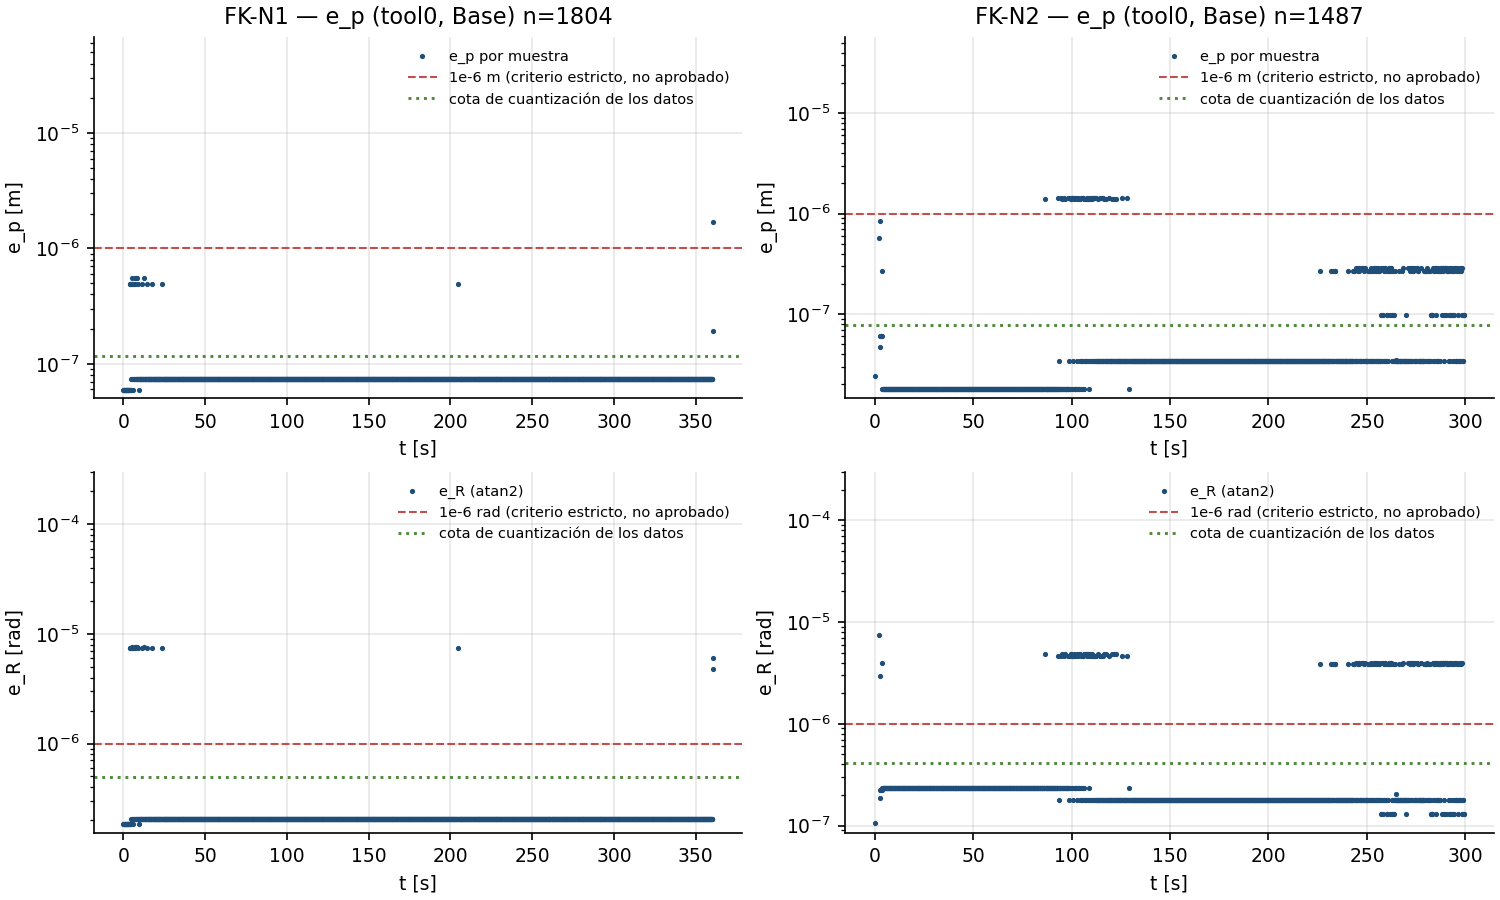
\includegraphics[width=0.92\textwidth]{../resultados/figuras/fk_real_errores_N1_N2.png}
\caption{Errores de FK propia frente al \texttt{robtarget} del IRC5 por muestra estacionaria, FK-N1 y FK-N2.}
\label{fig:fkreal}
\end{figure}

\subsection{Diagnósticos intencionales: TCP y orden articular}
\textbf{FK-D-TCP.} Con los datos de FK-N1 se comparó la FK propia con un TCP simulado en $z$ contra la \texttt{tool0} del controlador. El error de posición es igual a la longitud simulada más un residuo de $2{,}8\times10^{-8}$ m: 0,025 m para 0,025~m, 0,100 m para 0,100~m y 0,150 m para el TCP de 0,150~m. El coseno del ángulo entre el desplazamiento y el eje $z$ de la herramienta es $\ge0{,}99999999999$. Demuestra que comparar brida con TCP produce un error igual a la longitud de la herramienta y en el eje de la brida.

\textbf{FK-D-ORD.} Con datos de FK-N2 (149 muestras) se permutó $\mathbf{q}$ a propósito. Con $q_4\leftrightarrow q_6$ la mediana de $\ep$ es 0,125 m y $\eR$ 2,64 rad; con $q_1\leftrightarrow q_2$, 0,042 m y 0,120 rad; con orden invertido, 0,904 m y 1,49 rad; con rotación cíclica, 0,141 m y 1,30 rad. Al invertir la permutación el error vuelve a $\le1{,}43\times10^{-6}$ m y $\le4{,}87\times10^{-6}$ rad. Un error de orden articular se reconoce por una discrepancia grande que desaparece con la permutación inversa.

\begin{figure}[H]
\centering
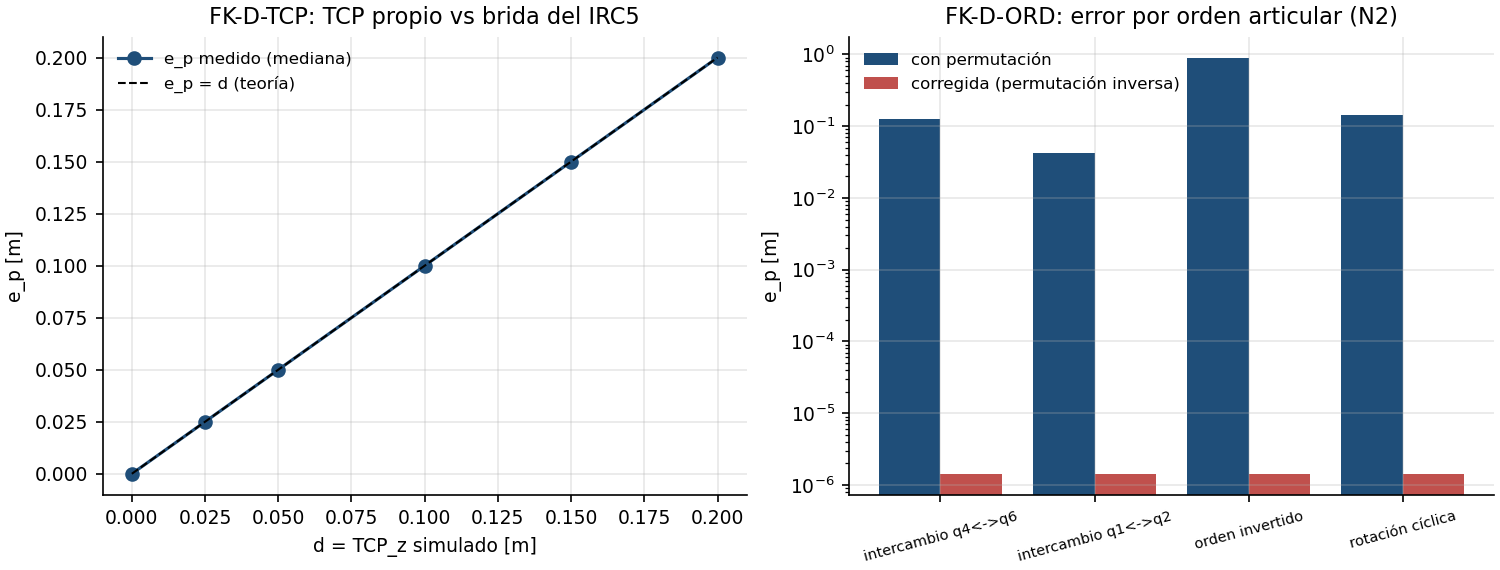
\includegraphics[width=0.92\textwidth]{../resultados/figuras/fk_d_tcp_d_ord.png}
\caption{Diagnósticos FK-D-TCP y FK-D-ORD (datos reales S1 con perturbación offline declarada).}
\end{figure}

\subsection{Diagnóstico de las 155 muestras FUERA y de las lecturas inválidas}
Los registros de las dos sesiones contienen 155 muestras con estado \texttt{FUERA} (32 en la sesión~1 y 123 en la sesión~2), según \ruta{hito3/datos/fk_real_procedencia.json}. Todas tienen $\Delta q=0$ y ventana $\le20$~ms. El diagnóstico, siguiendo el árbol del Bloque C, resulta:

% Generado por hito3.validacion; requiere \usepackage{booktabs,array}
\begin{table}[htbp]
\centering
\scriptsize
\setlength{\tabcolsep}{3pt}
\renewcommand{\arraystretch}{1.15}
\caption{Diagnóstico de las 155 muestras FUERA de las dos sesiones. Todas con $\Delta q=0$ y ventana $\le20$ ms. Mediana de $e_p$: 3.33e-07 m; máx. $e_R$: 1.32e-05 rad.}
\label{tab:fuera}
\begin{tabular}{p{11cm}r}
\toprule
\textbf{Clasificación (árbol del Bloque C)} & \textbf{Muestras} \\
\midrule
C: q id\'entico y pose del IRC5 distinta a la pose modal de esa q (indeterminada por datos) & 106 \\
D: pose modal repetida de esa q queda fuera de criterio (error reproducible; revisar pasos 2-6) & 23 \\
E: q con <3 lecturas estacionarias: sin pose modal con que contrastar (indeterminada por datos) & 26 \\
Lecturas inv\'alidas (ConnectTimeout/ConnectionError/ReadTimeout; sin datos q-pose) & 6263 \\
\bottomrule
\end{tabular}
\end{table}


Interpretación. En 116 de las 155 muestras solo falla la orientación frente a $10^{-6}$ rad y en 39 fallan posición y orientación. La mediana de $\ep$ es $3{,}33\times10^{-7}$ m; el máximo de $\eR$ es $1{,}32\times10^{-5}$ rad; el peor $\ep$ es $2{,}44\times10^{-6}$ m. La causa raíz queda \textbf{indeterminada por datos}: faltan un registro simultáneo y una repetición controlada. No se atribuye a ninguna causa. Estado P5 de FK-FUERA: \textit{parcial}.

Las 6263 lecturas inválidas (todas en la sesión~2: 6130 \texttt{ConnectTimeout}, 132 \texttt{ConnectionError}, 1 \texttt{ReadTimeout}) se extienden desde las 23:05 UTC del 04/11 hasta las 03:15 UTC del 05/11; no contienen par $\mathbf{q}$--pose y no se usaron en ninguna métrica. Se clasifican por tipo de excepción (caso FK-INV, \textit{parcial}). No se investigó el motivo del corte del enlace en ese periodo.

Nota de conteo. La tabla P1c cuenta 20 y 173 lecturas estacionarias fuera del criterio estricto (FK-N1 y FK-N2). La cifra no coincide con las 155 \texttt{FUERA} del registro porque P1c recalcula $\ep$ y $\eR$ (\texttt{arccos}) sobre todas las lecturas estacionarias de cada postura, incluidas las que la sesión había rotulado \texttt{NO\_EVALUABLE}. Recontado en \ruta{hito3/resultados/fk_real_errores_por_muestra.csv}: 101 muestras rotuladas \texttt{FUERA} son estacionarias y están en esas tablas (7 en N1 y 94 en N2), junto con 92 fuera del criterio entre las \texttt{NO\_EVALUABLE}. Esta reconciliación es cálculo del autor sobre el CSV; no figura en los resúmenes del paquete.

\begin{figure}[H]
\centering
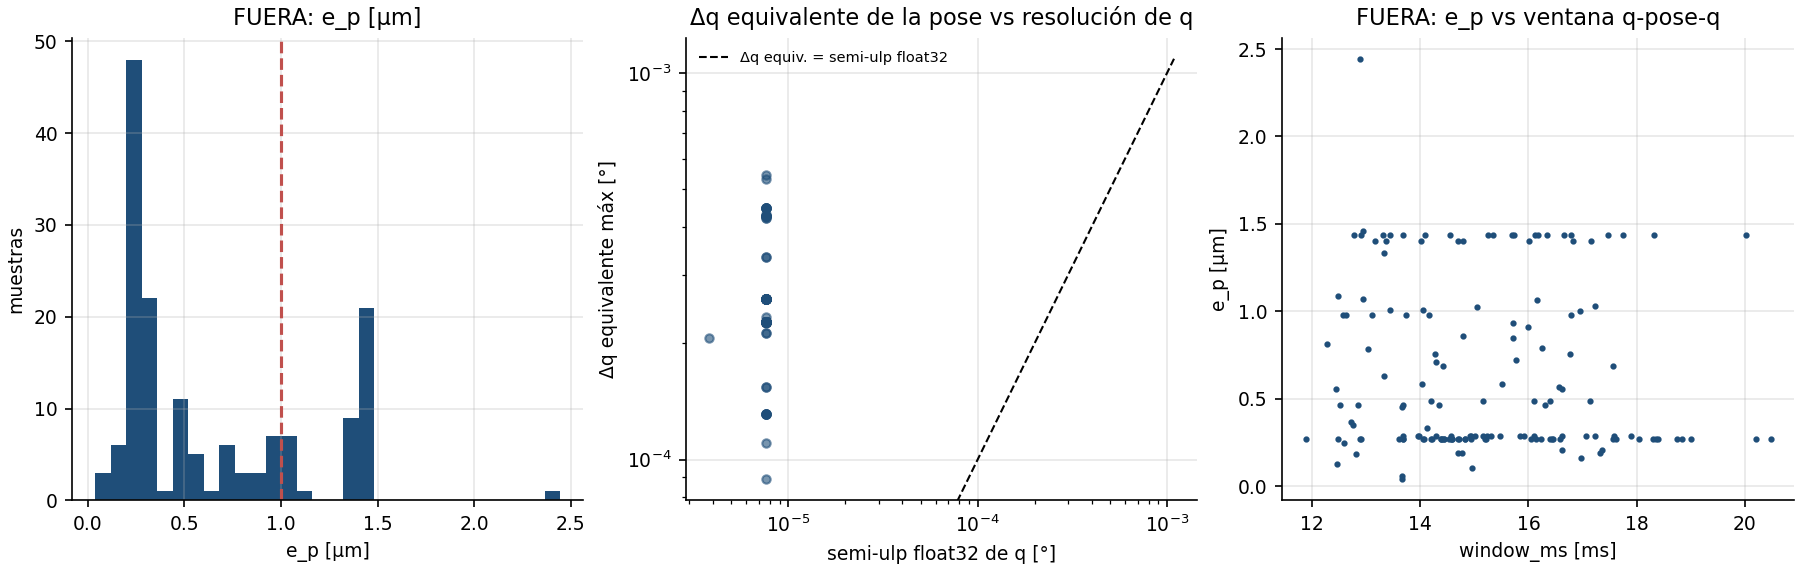
\includegraphics[width=0.92\textwidth]{../resultados/figuras/fk_fuera_diagnostico.png}
\caption{Diagnóstico de las muestras FUERA.}
\end{figure}

\subsection{Casos bloqueados}
FK-L-REAL (FK cerca de límites con datos reales) y FK-TCP-REAL (FK con el TCP físico) quedan \textit{bloqueados por acceso}: requieren permiso y hardware no disponibles en la sesión W14-S02 (NO-GO físico), y el plan alternativo es el offline ya presentado.

% ---------------------------------------------------------------- 5
\section{Cinemática inversa (Bloque D)}
\label{sec:ik}

La IK propia es analítica (Pieper para muñeca esférica, con \texttt{atan2}) y enumera las ocho ramas (frente/atrás, arriba/abajo, $q_5\pm$). No se exige $\mathbf{q}_{\mathrm{propia}}=\mathbf{q}_{\mathrm{ref}}$: cada rama se audita por su residuo de FK (propia e independiente), su pertenencia a límites de junta y su hallazgo por un DLS numérico independiente ($\lambda=10^{-3}$, tolerancia $10^{-9}$, $\le200$ iteraciones, $\le2$~s, semillas con \texttt{rng=12345}). Las poses objetivo salen de la FK sobre configuraciones documentadas.

\newgeometry{margin=1.2cm}
\begin{landscape}
% Generado por hito3.validacion; requiere \usepackage{booktabs,array,graphicx}
\begin{table}[htbp]
\centering
\scriptsize
\setlength{\tabcolsep}{3pt}
\renewcommand{\arraystretch}{1.15}
\caption{P2a. Poses objetivo de IK y métodos (propio: Pieper por \texttt{atan2}; referencia: DLS numérico sobre la FK de ROS-Industrial).}
\label{tab:P2a}
\resizebox{\linewidth}{!}{%
\begin{tabular}{llllllll}
\toprule
\textbf{ID pose} & \textbf{$T_d$ / fuente} & \textbf{Método propio} & \textbf{Método ref.} & \textbf{Semilla} & \textbf{DLS conv.} & \textbf{Ramas halladas} & \textbf{DLS sin rama} \\
\midrule
IK-1 & FK propia de q de FK-N1 (postura real S1 de la sesi\'on 1) & Pieper@b54ccfa & DLS(rosi) $\lambda$=0.001, tol=1e-09, it$\le$200, t$\le$2.0s & 34 semillas (rng=12345) & 34/34 & 8/8 & 0 \\
IK-2 & FK propia de q de FK-N2 (postura real S1 de la sesi\'on 2, q5$\approx$89.7$^\circ$) & Pieper@b54ccfa & DLS(rosi) $\lambda$=0.001, tol=1e-09, it$\le$200, t$\le$2.0s & 34 semillas (rng=12345) & 34/34 & 8/8 & 0 \\
IK-3 & FK propia de q sint\'etica con q5 = 0.5$^\circ$ (cerca de singularidad de mu\~neca) & Pieper@b54ccfa & DLS(rosi) $\lambda$=0.001, tol=1e-09, it$\le$200, t$\le$2.0s & 34 semillas (rng=12345) & 34/34 & 8/8 & 0 \\
IK-4 & FK propia de q sint\'etica con q5 = 0 exacto (singularidad de mu\~neca) & Pieper@b54ccfa & DLS(rosi) $\lambda$=0.001, tol=1e-09, it$\le$200, t$\le$2.0s & 34 semillas (rng=12345) & 34/34 & 8/8 & 0 \\
IK-5 & FK propia de q sint\'etica desplazada +0.8 m en x\_base (fuera del alcance) & Pieper@b54ccfa & DLS(rosi) $\lambda$=0.001, tol=1e-09, it$\le$200, t$\le$2.0s & 26 semillas (rng=12345) & 0/26 & 0/0 & 0 \\
\bottomrule
\end{tabular}
}
\end{table}

\end{landscape}
\restoregeometry

\textbf{Resumen por pose} (conteo de \ruta{hito3/resultados/ik_ramas.csv}, 40 ramas):
\begin{itemize}[leftmargin=*]
\item \textbf{IK-1} (postura FK-N1): 4 ramas \textit{válidas en modelo}, 4 \textit{no válidas} (violan el límite de J3).
\item \textbf{IK-2} (postura FK-N2, $q_5\approx89{,}7^\circ$): 1 válida; 7 no válidas por límites de J1, J3, J4 o J5. Aun así el DLS converge en 34/34 semillas.
\item \textbf{IK-3} (sintética, $q_5=0{,}5^\circ$, cerca de singularidad): 1 válida, 1 \textit{indeterminada por datos} (en un límite de junta las dos fuentes difieren en $3{,}3\times10^{-6}$ rad) y 6 no válidas.
\item \textbf{IK-4} ($q_5=0$ exacto, singularidad de muñeca): 2 ramas \textit{numéricamente singulares} ($q_4$ y $q_6$ solo quedan determinadas en suma) y 6 no válidas. Estado P5 \textit{parcial}: la familia continua de soluciones de la singularidad no se enumera.
\item \textbf{IK-5} (desplazada $+0{,}8$~m, fuera de alcance): 8 ramas \textit{sin solución: inexistente en el modelo} ($|\cos\theta_3|>1$) y DLS sin convergencia (0/26), con lo que se distingue \textit{inexistente} de \textit{no encontrada}.
\end{itemize}
Los residuos de FK de las ramas válidas y no válidas son del orden de $10^{-16}$ m y $0$ rad: una rama puede reproducir la pose y a la vez ser inadmisible por límites, lo que confirma que la igualdad de vectores articulares no es criterio de equivalencia. Los límites usados son los de la hoja ABB, no los leídos del controlador.

\begin{figure}[H]
\centering
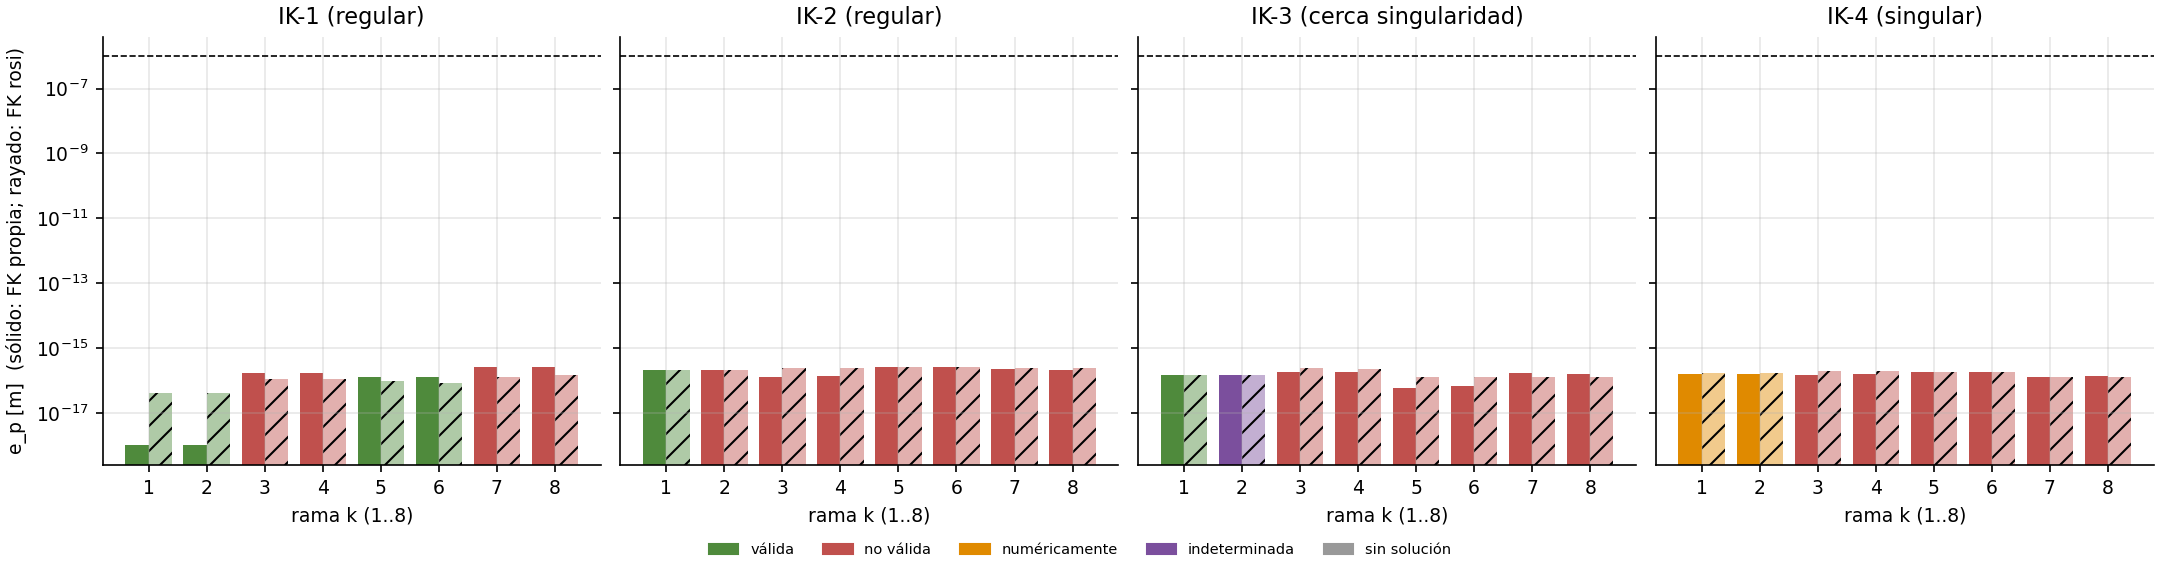
\includegraphics[width=0.92\textwidth]{../resultados/figuras/ik_ramas_residuos.png}
\caption{Residuos de FK por rama de IK y pose.}
\end{figure}

\newgeometry{margin=1.2cm}
\begin{landscape}
% Generado por hito3.validacion; requiere \usepackage{booktabs,longtable,array}
\begingroup
\scriptsize
\setlength{\tabcolsep}{2.5pt}
\renewcommand{\arraystretch}{1.12}
\begin{longtable}{lcllllllp{5.2cm}}
\caption{P2b. Las 8 ramas de Pieper por pose: residuos por FK propia y por FK independiente, límites y clasificación.}\label{tab:P2b}\\
\toprule
\textbf{ID pose} & \textbf{Rama $k$} & \textbf{Config.} & \textbf{$\mathbf{q}^{(k)}$ [rad]} & \textbf{$e_p/e_R$ FK propia [m/rad]} & \textbf{$e_p/e_R$ FK ref. [m/rad]} & \textbf{Límites} & \textbf{DLS} & \textbf{Estado de la solución} \\
\midrule
\endfirsthead
\toprule
\textbf{ID pose} & \textbf{Rama $k$} & \textbf{Config.} & \textbf{$\mathbf{q}^{(k)}$ [rad]} & \textbf{$e_p/e_R$ FK propia [m/rad]} & \textbf{$e_p/e_R$ FK ref. [m/rad]} & \textbf{Límites} & \textbf{DLS} & \textbf{Estado de la solución} \\
\midrule
\endhead
\bottomrule
\endfoot
IK-1 & 1 & fre/arr/q5+ & $[-1.278,\,-0.212,\,0.173,\,1.604,\,0.5541,\,-2.347]$ & $0$ / $0$ & $4.2\times10^{-17}$ / $0$ & s\'i & sí & v\'alida en modelo \\
IK-1 & 2 & fre/arr/q5- & $[-1.278,\,-0.212,\,0.173,\,-1.538,\,-0.5541,\,0.7941]$ & $0$ / $0$ & $4.2\times10^{-17}$ / $0$ & s\'i & sí & v\'alida en modelo \\
IK-1 & 3 & fre/aba/q5+ & $[-1.278,\,1.434,\,-2.859,\,0.5633,\,1.396,\,-0.8472]$ & $1.7\times10^{-16}$ / $0$ & $1.1\times10^{-16}$ / $0$ & no: J3 & sí & no v\'alida (viola l\'imites de junta J3) \\
IK-1 & 4 & fre/aba/q5- & $[-1.278,\,1.434,\,-2.859,\,-2.578,\,-1.396,\,2.294]$ & $1.7\times10^{-16}$ / $0$ & $1.1\times10^{-16}$ / $0$ & no: J3 & sí & no v\'alida (viola l\'imites de junta J3) \\
IK-1 & 5 & atr/arr/q5+ & $[1.864,\,-1.434,\,0.173,\,-2.574,\,1.783,\,-0.6045]$ & $1.3\times10^{-16}$ / $0$ & $9.7\times10^{-17}$ / $0$ & s\'i & sí & v\'alida en modelo \\
IK-1 & 6 & atr/arr/q5- & $[1.864,\,-1.434,\,0.173,\,0.568,\,-1.783,\,-3.746]$ & $1.3\times10^{-16}$ / $0$ & $8.3\times10^{-17}$ / $0$ & s\'i & sí & v\'alida en modelo \\
IK-1 & 7 & atr/aba/q5+ & $[1.864,\,0.212,\,-2.859,\,-2.169,\,0.69,\,-1.585]$ & $2.6\times10^{-16}$ / $0$ & $1.3\times10^{-16}$ / $0$ & no: J3 & sí & no v\'alida (viola l\'imites de junta J3) \\
IK-1 & 8 & atr/aba/q5- & $[1.864,\,0.212,\,-2.859,\,0.9724,\,-0.69,\,1.557]$ & $2.6\times10^{-16}$ / $0$ & $1.4\times10^{-16}$ / $0$ & no: J3 & sí & no v\'alida (viola l\'imites de junta J3) \\
IK-2 & 1 & fre/arr/q5+ & $[0.05143,\,-0.03364,\,0.04518,\,-0.228,\,1.565,\,-2.338]$ & $2.1\times10^{-16}$ / $0$ & $2.0\times10^{-16}$ / $0$ & s\'i & sí & v\'alida en modelo \\
IK-2 & 2 & fre/arr/q5- & $[0.05143,\,-0.03364,\,0.04518,\,2.914,\,-1.565,\,0.8032]$ & $2.1\times10^{-16}$ / $0$ & $2.1\times10^{-16}$ / $0$ & no: J4 & sí & no v\'alida (viola l\'imites de junta J4) \\
IK-2 & 3 & fre/aba/q5+ & $[0.05143,\,1.469,\,-2.731,\,-0.6605,\,2.764,\,-2.965]$ & $1.2\times10^{-16}$ / $0$ & $2.3\times10^{-16}$ / $0$ & no: J3,J5 & sí & no v\'alida (viola l\'imites de junta J3,J5) \\
IK-2 & 4 & fre/aba/q5- & $[0.05143,\,1.469,\,-2.731,\,2.481,\,-2.764,\,0.1763]$ & $1.3\times10^{-16}$ / $0$ & $2.4\times10^{-16}$ / $0$ & no: J3,J5 & sí & no v\'alida (viola l\'imites de junta J3,J5) \\
IK-2 & 5 & atr/arr/q5+ & $[-3.09,\,-1.469,\,0.04518,\,0.992,\,2.868,\,1.776]$ & $2.6\times10^{-16}$ / $0$ & $2.6\times10^{-16}$ / $2.1\times10^{-8}$ & no: J1,J5 & sí & no v\'alida (viola l\'imites de junta J1,J5) \\
IK-2 & 6 & atr/arr/q5- & $[-3.09,\,-1.469,\,0.04518,\,-2.15,\,-2.868,\,-1.365]$ & $2.6\times10^{-16}$ / $0$ & $2.6\times10^{-16}$ / $0$ & no: J1,J5 & sí & no v\'alida (viola l\'imites de junta J1,J5) \\
IK-2 & 7 & atr/aba/q5+ & $[-3.09,\,0.03364,\,-2.731,\,2.889,\,2.008,\,-2.448]$ & $2.3\times10^{-16}$ / $2.1\times10^{-8}$ & $2.5\times10^{-16}$ / $0$ & no: J1,J3,J4 & sí & no v\'alida (viola l\'imites de junta J1,J3,J4) \\
IK-2 & 8 & atr/aba/q5- & $[-3.09,\,0.03364,\,-2.731,\,-0.2522,\,-2.008,\,0.6932]$ & $2.2\times10^{-16}$ / $0$ & $2.4\times10^{-16}$ / $0$ & no: J1,J3 & sí & no v\'alida (viola l\'imites de junta J1,J3) \\
IK-3 & 1 & fre/arr/q5+ & $[0.1745,\,0.5236,\,-0.1745,\,0.3491,\,0.008727,\,0.6981]$ & $1.5\times10^{-16}$ / $0$ & $1.5\times10^{-16}$ / $0$ & s\'i & sí & v\'alida en modelo \\
IK-3 & 2 & fre/arr/q5- & $[0.1745,\,0.5236,\,-0.1745,\,-2.793,\,-0.008727,\,3.84]$ & $1.5\times10^{-16}$ / $0$ & $1.5\times10^{-16}$ / $0$ & s\'i & sí & indeterminada por datos (l\'imite de junta: las fuentes difieren en 3.3e-06 rad) \\
IK-3 & 3 & fre/aba/q5+ & $[0.1745,\,1.783,\,-2.512,\,0.003374,\,1.086,\,1.046]$ & $1.8\times10^{-16}$ / $0$ & $2.4\times10^{-16}$ / $0$ & no: J3 & sí & no v\'alida (viola l\'imites de junta J3) \\
IK-3 & 4 & fre/aba/q5- & $[0.1745,\,1.783,\,-2.512,\,-3.138,\,-1.086,\,-2.096]$ & $1.8\times10^{-16}$ / $0$ & $2.3\times10^{-16}$ / $0$ & no: J3,J4 & sí & no v\'alida (viola l\'imites de junta J3,J4) \\
IK-3 & 5 & atr/arr/q5+ & $[-2.967,\,-1.783,\,-0.1745,\,-3.139,\,1.541,\,1.047]$ & $5.7\times10^{-17}$ / $0$ & $1.2\times10^{-16}$ / $0$ & no: J1,J4 & sí & no v\'alida (viola l\'imites de junta J1,J4) \\
IK-3 & 6 & atr/arr/q5- & $[-2.967,\,-1.783,\,-0.1745,\,0.002986,\,-1.541,\,-2.094]$ & $6.9\times10^{-17}$ / $0$ & $1.3\times10^{-16}$ / $0$ & no: J1 & sí & no v\'alida (viola l\'imites de junta J1) \\
IK-3 & 7 & atr/aba/q5+ & $[-2.967,\,-0.5236,\,-2.512,\,-3.135,\,0.4637,\,1.041]$ & $1.7\times10^{-16}$ / $2.1\times10^{-8}$ & $1.3\times10^{-16}$ / $0$ & no: J1,J3,J4 & sí & no v\'alida (viola l\'imites de junta J1,J3,J4) \\
IK-3 & 8 & atr/aba/q5- & $[-2.967,\,-0.5236,\,-2.512,\,0.006673,\,-0.4637,\,-2.1]$ & $1.6\times10^{-16}$ / $0$ & $1.3\times10^{-16}$ / $0$ & no: J1,J3 & sí & no v\'alida (viola l\'imites de junta J1,J3) \\
IK-4 & 1 & fre/arr/q5+ & $[0.1745,\,0.5236,\,-0.1745,\,0.3491,\,0,\,0.6981]$ & $1.6\times10^{-16}$ / $0$ & $1.7\times10^{-16}$ / $0$ & s\'i & sí & num\'ericamente singular (q4 y q6 solo determinados en suma) \\
IK-4 & 2 & fre/arr/q5- & $[0.1745,\,0.5236,\,-0.1745,\,-2.793,\,0,\,3.84]$ & $1.6\times10^{-16}$ / $0$ & $1.7\times10^{-16}$ / $0$ & s\'i & sí & num\'ericamente singular (q4 y q6 solo determinados en suma) \\
IK-4 & 3 & fre/aba/q5+ & $[0.1745,\,1.783,\,-2.512,\,2.09e-16,\,1.077,\,1.047]$ & $1.5\times10^{-16}$ / $0$ & $2.0\times10^{-16}$ / $0$ & no: J3 & sí & no v\'alida (viola l\'imites de junta J3) \\
IK-4 & 4 & fre/aba/q5- & $[0.1745,\,1.783,\,-2.512,\,-3.142,\,-1.077,\,-2.094]$ & $1.6\times10^{-16}$ / $0$ & $2.0\times10^{-16}$ / $0$ & no: J3,J4 & sí & no v\'alida (viola l\'imites de junta J3,J4) \\
IK-4 & 5 & atr/arr/q5+ & $[-2.967,\,-1.783,\,-0.1745,\,-3.142,\,1.533,\,1.047]$ & $1.8\times10^{-16}$ / $0$ & $1.8\times10^{-16}$ / $0$ & no: J1,J4 & sí & no v\'alida (viola l\'imites de junta J1,J4) \\
IK-4 & 6 & atr/arr/q5- & $[-2.967,\,-1.783,\,-0.1745,\,1.469e-16,\,-1.533,\,-2.094]$ & $1.8\times10^{-16}$ / $0$ & $1.8\times10^{-16}$ / $0$ & no: J1 & sí & no v\'alida (viola l\'imites de junta J1) \\
IK-4 & 7 & atr/aba/q5+ & $[-2.967,\,-0.5236,\,-2.512,\,-3.142,\,0.4555,\,1.047]$ & $1.3\times10^{-16}$ / $2.1\times10^{-8}$ & $1.3\times10^{-16}$ / $0$ & no: J1,J3,J4 & sí & no v\'alida (viola l\'imites de junta J1,J3,J4) \\
IK-4 & 8 & atr/aba/q5- & $[-2.967,\,-0.5236,\,-2.512,\,4.357e-16,\,-0.4555,\,-2.094]$ & $1.4\times10^{-16}$ / $0$ & $1.3\times10^{-16}$ / $0$ & no: J1,J3 & sí & no v\'alida (viola l\'imites de junta J1,J3) \\
IK-5 & 1 & fre/arr/q5+ & n/d & n/d & n/d & n/a & no & sin soluci\'on: inexistente en el modelo (|cos $\theta$3| > 1: pose fuera del alcance de la rama) \\
IK-5 & 2 & fre/arr/q5- & n/d & n/d & n/d & n/a & no & sin soluci\'on: inexistente en el modelo (|cos $\theta$3| > 1: pose fuera del alcance de la rama) \\
IK-5 & 3 & fre/aba/q5+ & n/d & n/d & n/d & n/a & no & sin soluci\'on: inexistente en el modelo (|cos $\theta$3| > 1: pose fuera del alcance de la rama) \\
IK-5 & 4 & fre/aba/q5- & n/d & n/d & n/d & n/a & no & sin soluci\'on: inexistente en el modelo (|cos $\theta$3| > 1: pose fuera del alcance de la rama) \\
IK-5 & 5 & atr/arr/q5+ & n/d & n/d & n/d & n/a & no & sin soluci\'on: inexistente en el modelo (|cos $\theta$3| > 1: pose fuera del alcance de la rama) \\
IK-5 & 6 & atr/arr/q5- & n/d & n/d & n/d & n/a & no & sin soluci\'on: inexistente en el modelo (|cos $\theta$3| > 1: pose fuera del alcance de la rama) \\
IK-5 & 7 & atr/aba/q5+ & n/d & n/d & n/d & n/a & no & sin soluci\'on: inexistente en el modelo (|cos $\theta$3| > 1: pose fuera del alcance de la rama) \\
IK-5 & 8 & atr/aba/q5- & n/d & n/d & n/d & n/a & no & sin soluci\'on: inexistente en el modelo (|cos $\theta$3| > 1: pose fuera del alcance de la rama) \\
\end{longtable}
{\tiny Límites: de la hoja ABB (\texttt{dh.py}); xacro y URDF difieren hasta $3.3\times10^{-6}$ rad. Cribado exploratorio: $e_p\le10^{-6}$ m, $e_R\le10^{-5}$ rad (pendiente de aprobación).}
\endgroup

\end{landscape}
\restoregeometry

IK-1 a IK-3 y IK-5 quedan \textit{verificados} (S0, procedimental) e IK-4 \textit{parcial}. IK-REAL (IK con movimiento físico) está \textit{bloqueado por acceso}: S3 no alcanzado y plan alternativo offline.

% ---------------------------------------------------------------- 6
\section{Jacobiano y diferencias finitas (Bloque E)}
\label{sec:jac}

Convención: twist $[v;\omega]$ (lineal arriba), expresado en la base $\{B\}$, con columnas $J_i=\bigl[z_{i-1}\times(p_{TCP}-o_{i-1});\,z_{i-1}\bigr]$. Como $J_v$ está en m/rad y $J_\omega$ en rad/rad, los errores se reportan por separado:
\begin{equation}
e_{J_v}=\lVert J_{v,\mathrm{propio}}-J_{v,\mathrm{ref}}\rVert_F\ [\mathrm{m/rad}],\qquad
e_{J_\omega}=\lVert J_{\omega,\mathrm{propio}}-J_{\omega,\mathrm{ref}}\rVert_F\ [\mathrm{rad/rad}].
\end{equation}
La referencia es la diferenciación central de la FK de ROS-Industrial, $\bigl(p(\mathbf{q}+h\mathbf{e}_i)-p(\mathbf{q}-h\mathbf{e}_i)\bigr)/2h$ con $h=10^{-5}$ rad, para el punto \texttt{tool0} y para el TCP de 0,150~m. Se evaluó en las dos posturas reales, en una postura sintética regular (J-N3) y en una cerca de límites (J-N4), con $\dot{\mathbf{q}}_{test}=[0{,}1;-0{,}2;0{,}15;0{,}3;-0{,}25;0{,}4]$ rad/s.

\newgeometry{margin=1.2cm}
\begin{landscape}
% Generado por hito3.validacion; requiere \usepackage{booktabs,array,graphicx}
\begin{table}[htbp]
\centering
\scriptsize
\setlength{\tabcolsep}{3pt}
\renewcommand{\arraystretch}{1.15}
\caption{P3a. Jacobiano propio frente a referencia independiente (FD central sobre la FK de ROS-Industrial, $h=1e-05$ rad). $\dot{q}_{test}=[0.1, -0.2, 0.15, 0.3, -0.25, 0.4]$ rad/s. Errores de $J_v$ y $J_\omega$ por separado.}
\label{tab:P3a}
\resizebox{\linewidth}{!}{%
\begin{tabular}{llllllll}
\toprule
\textbf{ID} & \textbf{$\mathbf{q}$ [rad]} & \textbf{Frame/TCP/Twist} & \textbf{$e_{J_v}$ [m/rad]} & \textbf{$e_{J_\omega}$ [rad/rad]} & \textbf{$\lVert J\dot q-\mathrm{FD}\rVert$ lin./ang.} & \textbf{$J\dot{\mathbf{q}}$ [m/s, rad/s]} & \textbf{Decisión} \\
\midrule
J-N1-tcp & $[-1.278,\,-0.212,\,0.173,\,1.604,\,0.5541,\,-2.347]$ & B; TCP; [v;w] & $1.2\times10^{-11}$ & $1.8\times10^{-11}$ & $6.7\times10^{-11}$ / $2.9\times10^{-10}$ & $[-0.0169,\,0.038,\,0.0476,\,0.349,\,-0.573,\,-0.118]$ & verificado \\
J-N1-tool0 & $[-1.278,\,-0.212,\,0.173,\,1.604,\,0.5541,\,-2.347]$ & B; tool0; [v;w] & $9.2\times10^{-12}$ & $1.8\times10^{-11}$ & $7.6\times10^{-11}$ / $2.9\times10^{-10}$ & $[-0.000932,\,0.0538,\,0.0179,\,0.349,\,-0.573,\,-0.118]$ & verificado \\
J-N2-tcp & $[0.05143,\,-0.03364,\,0.04518,\,-0.228,\,1.565,\,-2.338]$ & B; TCP; [v;w] & $8.0\times10^{-12}$ & $9.7\times10^{-12}$ & $5.6\times10^{-11}$ / $1.9\times10^{-10}$ & $[0.009,\,0.0948,\,-0.00211,\,0.318,\,-0.368,\,-0.237]$ & verificado \\
J-N2-tool0 & $[0.05143,\,-0.03364,\,0.04518,\,-0.228,\,1.565,\,-2.338]$ & B; tool0; [v;w] & $7.8\times10^{-12}$ & $9.7\times10^{-12}$ & $4.2\times10^{-11}$ / $1.9\times10^{-10}$ & $[-0.0368,\,0.0486,\,0.00832,\,0.318,\,-0.368,\,-0.237]$ & verificado \\
J-N3-tcp & $[0.3,\,-0.5,\,0.6,\,-0.8,\,1.1,\,0.4]$ & B; TCP; [v;w] & $1.0\times10^{-11}$ & $1.6\times10^{-11}$ & $7.4\times10^{-11}$ / $6.4\times10^{-11}$ & $[-0.00731,\,0.0876,\,-0.036,\,0.593,\,-0.319,\,-0.0167]$ & verificado \\
J-N3-tool0 & $[0.3,\,-0.5,\,0.6,\,-0.8,\,1.1,\,0.4]$ & B; tool0; [v;w] & $8.5\times10^{-12}$ & $1.6\times10^{-11}$ & $8.6\times10^{-11}$ / $6.4\times10^{-11}$ & $[-0.0378,\,0.03,\,-0.0188,\,0.593,\,-0.319,\,-0.0167]$ & verificado \\
J-N4-tcp & $[2.793,\,-1.833,\,1.134,\,-2.705,\,2.007,\,-6.894]$ & B; TCP; [v;w] & $8.9\times10^{-12}$ & $4.2\times10^{-11}$ & $8.6\times10^{-11}$ / $2.5\times10^{-10}$ & $[-0.0134,\,0.102,\,-0.0232,\,0.16,\,-0.0831,\,0.517]$ & verificado \\
J-N4-tool0 & $[2.793,\,-1.833,\,1.134,\,-2.705,\,2.007,\,-6.894]$ & B; tool0; [v;w] & $6.0\times10^{-12}$ & $4.2\times10^{-11}$ & $5.2\times10^{-11}$ / $2.5\times10^{-10}$ & $[-0.00364,\,0.0381,\,-0.0365,\,0.16,\,-0.0831,\,0.517]$ & verificado \\
\bottomrule
\end{tabular}
}
\end{table}

\end{landscape}
\restoregeometry

\textbf{Resultado.} $e_{J_v}$ entre $6{,}0\times10^{-12}$ y $1{,}2\times10^{-11}$ m/rad y $e_{J_\omega}$ entre $9{,}7\times10^{-12}$ y $4{,}2\times10^{-11}$ rad/rad. Estas diferencias están dominadas por el error de la propia diferenciación numérica, no por el Jacobiano analítico (así lo indica la curva siguiente). La velocidad $J\dot{\mathbf{q}}$ coincide con la diferencia finita a $\lesssim9\times10^{-11}$ m/s y $\lesssim3\times10^{-10}$ rad/s. Cabe observar que $J_\omega$ no depende del punto elegido: coincide en \texttt{tool0} y TCP, mientras que $J_v$ cambia (los vectores $J\dot{\mathbf{q}}$ lineales difieren entre ambas columnas de la tabla).

\subsection{Curva $h\to E(h)$}
Para caracterizar la referencia se barrió $h$ entre $10^{-1}$ y $10^{-10}$ rad en la postura de FK-N2.

% Generado por hito3.validacion; requiere \usepackage{booktabs,array,graphicx}
\begin{table}[htbp]
\centering
\scriptsize
\setlength{\tabcolsep}{3pt}
\renewcommand{\arraystretch}{1.15}
\caption{P3b. Curva $h\to E_i(h)$ en la postura de FK-N2 (TCP). Mínimo estable observado $h^*=1e-05$ rad; pendientes log-log 2.00 (truncamiento) y -1.18 (redondeo).}
\label{tab:P3b}
\resizebox{\linewidth}{!}{%
\begin{tabular}{lrrrrrrrr}
\toprule
\textbf{$h$ [rad]} & \textbf{$E_{J_v}$ [m/rad]} & \textbf{$E_{J_\omega}$ [rad/rad]} & \textbf{$E_1$} & \textbf{$E_2$} & \textbf{$E_3$} & \textbf{$E_4$} & \textbf{$E_5$} & \textbf{$E_6$} \\
\midrule
$0.1$ & $0.00105$ & $1.57\times10^{-15}$ & $4.9\times10^{-4}$ & $5.3\times10^{-4}$ & $5.6\times10^{-4}$ & $3.7\times10^{-4}$ & $3.7\times10^{-4}$ & $3.3\times10^{-17}$ \\
$0.01$ & $1.05\times10^{-5}$ & $1.90\times10^{-14}$ & $4.9\times10^{-6}$ & $5.3\times10^{-6}$ & $5.6\times10^{-6}$ & $3.7\times10^{-6}$ & $3.7\times10^{-6}$ & $1.5\times10^{-17}$ \\
$0.001$ & $1.05\times10^{-7}$ & $1.48\times10^{-13}$ & $4.9\times10^{-8}$ & $5.3\times10^{-8}$ & $5.6\times10^{-8}$ & $3.7\times10^{-8}$ & $3.7\times10^{-8}$ & $1.5\times10^{-17}$ \\
$1.0\times10^{-4}$ & $1.05\times10^{-9}$ & $1.98\times10^{-12}$ & $4.9\times10^{-10}$ & $5.3\times10^{-10}$ & $5.6\times10^{-10}$ & $3.7\times10^{-10}$ & $3.7\times10^{-10}$ & $1.5\times10^{-17}$ \\
$1.0\times10^{-5}$ & $7.96\times10^{-12}$ & $9.71\times10^{-12}$ & $4.4\times10^{-12}$ & $3.3\times10^{-12}$ & $2.5\times10^{-12}$ & $4.6\times10^{-12}$ & $2.4\times10^{-12}$ & $1.5\times10^{-17}$ \\
$1.0\times10^{-6}$ & $9.57\times10^{-11}$ & $1.52\times10^{-10}$ & $3.2\times10^{-11}$ & $7.8\times10^{-11}$ & $2.4\times10^{-11}$ & $2.2\times10^{-11}$ & $3.2\times10^{-11}$ & $1.5\times10^{-17}$ \\
$1.0\times10^{-7}$ & $1.26\times10^{-9}$ & $1.71\times10^{-9}$ & $6.1\times10^{-10}$ & $4.9\times10^{-10}$ & $6.5\times10^{-10}$ & $5.6\times10^{-10}$ & $4.9\times10^{-10}$ & $1.5\times10^{-17}$ \\
$1.0\times10^{-8}$ & $5.27\times10^{-9}$ & $8.63\times10^{-9}$ & $2.4\times10^{-9}$ & $2.0\times10^{-9}$ & $3.4\times10^{-9}$ & $2.3\times10^{-9}$ & $10.0\times10^{-10}$ & $1.5\times10^{-17}$ \\
$1.0\times10^{-9}$ & $8.06\times10^{-8}$ & $1.17\times10^{-7}$ & $4.6\times10^{-8}$ & $4.6\times10^{-8}$ & $2.9\times10^{-8}$ & $5.4\times10^{-9}$ & $3.8\times10^{-8}$ & $1.5\times10^{-17}$ \\
$1.0\times10^{-10}$ & $1.22\times10^{-6}$ & $5.66\times10^{-7}$ & $1.4\times10^{-7}$ & $5.7\times10^{-7}$ & $8.1\times10^{-7}$ & $4.2\times10^{-7}$ & $5.7\times10^{-7}$ & $1.5\times10^{-17}$ \\
\bottomrule
\end{tabular}
}
\end{table}


El error baja con pendiente log-log 2,00 (truncamiento, $O(h^2)$) hasta un mínimo estable en $h^*=10^{-5}$ rad ($E_{J_v}=7{,}96\times10^{-12}$ m/rad) y sube con pendiente $-1{,}18$ para $h$ menores (cancelación, $O(\epsilon/h)$). La columna $E_6$ es constante (del orden de $10^{-17}$) porque $q_6$ no mueve la posición de \texttt{tool0}/TCP situados en su eje.

\begin{figure}[H]
\centering
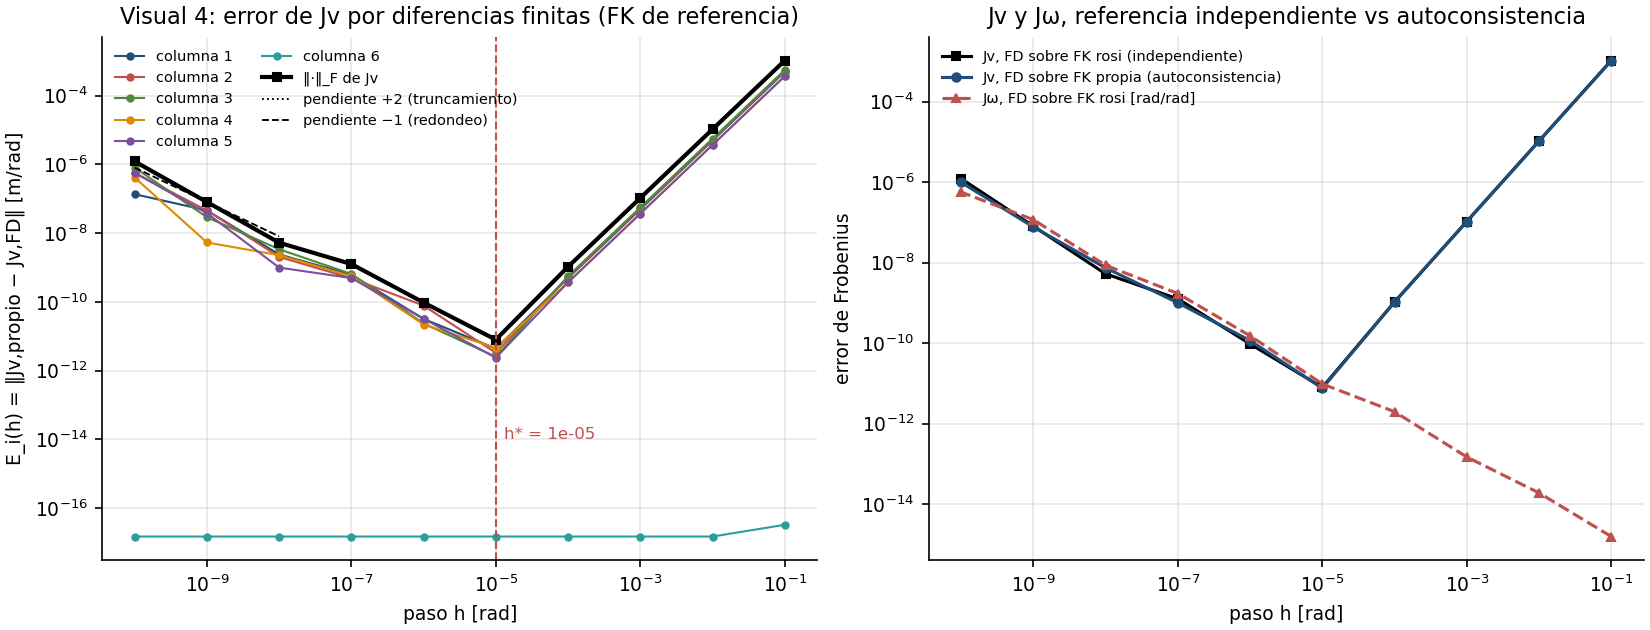
\includegraphics[width=0.78\textwidth]{../resultados/figuras/jacobiano_fd_curva_visual4.png}
\caption{Error de $J_v$ por diferencias finitas en función de $h$ (equivale al Visual~4 del documento oficial).}
\end{figure}
\begin{figure}[H]
\centering
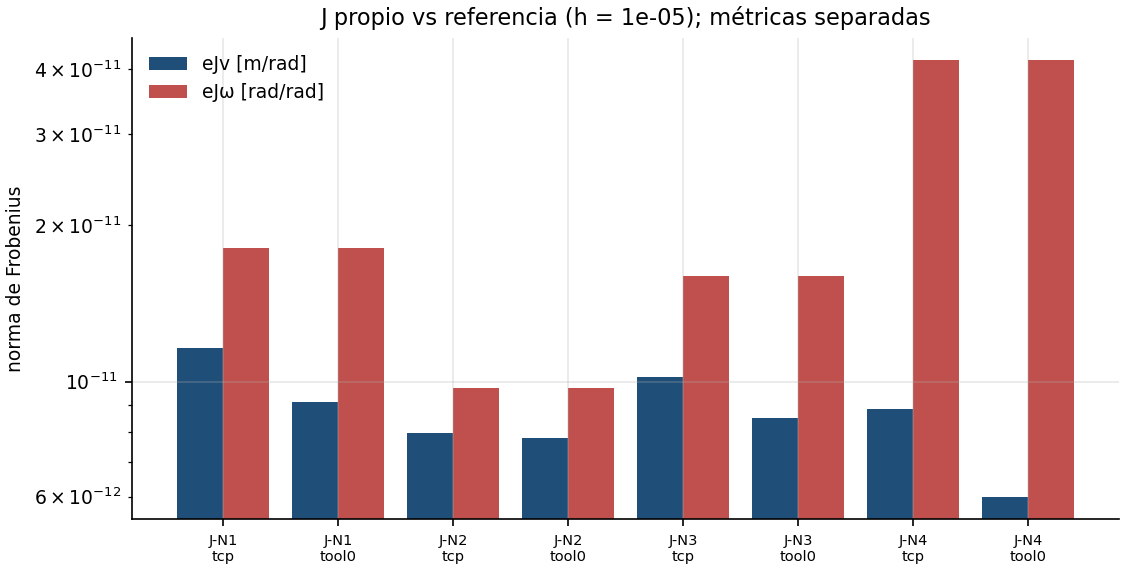
\includegraphics[width=0.78\textwidth]{../resultados/figuras/jacobiano_errores_separados.png}
\caption{$e_{J_v}$ y $e_{J_\omega}$ por separado para los cuatro casos.}
\end{figure}

J-N1 a J-N4 y J-FD quedan \textit{verificados} (S0, procedimental). J-REAL (Jacobiano frente al controlador) está \textit{bloqueado por acceso}: depende de hardware y GO. No se comparó $J$ con un Jacobiano del controlador ni de MoveIt; la referencia es numérica sobre la FK independiente.

% ---------------------------------------------------------------- 7
\section{Singularidades y esfuerzo (Bloque F)}
\label{sec:sing}

Se analiza la matriz escalada $J_s=[J_v/L;\,J_\omega]$ con $L=0{,}58$~m y el umbral de rango numérico $\tau_{num}=\max(m,n)\,\epsilon_{mach}\,\sigma_{\max}$. El subespacio es la tarea completa de 6 grados de libertad en el TCP. El condicionamiento del $J$ sin escalar mezcla unidades y no se interpreta. Para el esfuerzo estático se aplica $F=10$~N hacia abajo en el TCP y se compara $J^{T}F$ con $\tau_{act}=M\ddot{\mathbf{q}}+C\dot{\mathbf{q}}+g$ con $\dot{\mathbf{q}}$, $\ddot{\mathbf{q}}$ declarados.

% Generado por hito3.validacion; requiere \usepackage{booktabs,array,graphicx}
\begin{table}[htbp]
\centering
\scriptsize
\setlength{\tabcolsep}{3pt}
\renewcommand{\arraystretch}{1.15}
\caption{P4. Análisis de singularidad (SVD de $J_s$). $\tau_{num}=\max(m,n)\,\epsilon\,\sigma_{\max}$; $F$ = 10 N hacia abajo en el TCP; $\tau_{act}=M\ddot q+C\dot q+g$ con $\dot q,\ddot q$ declarados. El $\kappa$ de $J$ sin escalar mezcla unidades y no se interpreta.}
\label{tab:P4}
\resizebox{\linewidth}{!}{%
\begin{tabular}{llllllllllr}
\toprule
\textbf{ID} & \textbf{Subespacio} & \textbf{Escala} & \textbf{rango/$r_{\max}$} & \textbf{$\sigma_{\min}/\sigma_{\max}$} & \textbf{$\tau_{num}$} & \textbf{$\mathbf{q}$ [rad]} & \textbf{Dir. perdida $[v;\omega]$ (unit.)} & \textbf{$1/\sigma_{\min}$} & \textbf{$\lVert J^TF\rVert/\lVert\tau_{act}\rVert$ [N m]} & \textbf{$\kappa(J_s)$} \\
\midrule
F-reg & 6D TCP & $L=0.58$ m & 6/6 & $0.076$ & $2.6\times10^{-15}$ & $[-1.278,\,-0.212,\,0.173,\,1.604,\,0.5541,\,-2.347]$ & $[-0.022,\,0.014,\,0.57,\,0.64,\,0.52,\,0.013]$ & $6.7$ & $6.61$ / $9.65$ & $13$ \\
F-q5 & 6D TCP & $L=0.58$ m & 6/6 & $0.0013$ & $2.6\times10^{-15}$ & $[-1.278,\,-0.212,\,0.173,\,1.604,\,0.008727,\,-2.347]$ & $[-0.054,\,0.1,\,0.52,\,0.81,\,0.25,\,0.03]$ & $4.1e+02$ & $6.98$ / $9.67$ & $7.9e+02$ \\
F-q5-0 & 6D TCP & $L=0.58$ m & 5/6 & $4.1\times10^{-17}$ & $2.6\times10^{-15}$ & $[-1.278,\,-0.212,\,0.173,\,1.604,\,0,\,-2.347]$ & $[-0.054,\,0.1,\,0.52,\,0.81,\,0.24,\,0.031]$ & $1.3\times10^{16}$ & $6.98$ / $9.67$ & $2.4\times10^{16}$ \\
F-codo & 6D TCP & $L=0.58$ m & 5/6 & $3.2\times10^{-17}$ & $2.9\times10^{-15}$ & $[-1.278,\,0.35,\,-1.343,\,0.5,\,0.9,\,0.3]$ & $[0.085,\,-0.28,\,0.81,\,0.38,\,0.33,\,0.073]$ & $1.4\times10^{16}$ & $5.52$ / $9.85$ & $3.1\times10^{16}$ \\
F-hombro & 6D TCP & $L=0.58$ m & 5/6 & $7.5\times10^{-17}$ & $2.7\times10^{-15}$ & $[-1.278,\,-0.5236,\,-0.3689,\,0.5,\,0.9,\,0.3]$ & $[-0.82,\,-0.25,\,-8.5e-17,\,-0.0086,\,0.028,\,0.52]$ & $6.5\times10^{15}$ & $4.53$ / $9.38$ & $1.3\times10^{16}$ \\
\bottomrule
\end{tabular}
}
\end{table}


\textbf{Hallazgos.}
\begin{itemize}[leftmargin=*]
\item \textbf{Regular (F-reg).} Rango 6/6, $\sigma_{\min}/\sigma_{\max}=0{,}076$, $\kappa(J_s)=13$.
\item \textbf{Cerca de la singularidad de muñeca (F-q5, $q_5=0{,}5^\circ$).} Rango aún 6/6 pero $\sigma_{\min}/\sigma_{\max}=0{,}0013$ y $\kappa=7{,}9\times10^{2}$; el factor de amplificación $1/\sigma_{\min}$ crece a $4{,}1\times10^{2}$.
\item \textbf{Singularidades exactas (F-q5-0, F-codo, F-hombro).} Rango 5/6 con $\sigma_{\min}/\sigma_{\max}\approx10^{-17}$, por debajo de $\tau_{num}\approx3\times10^{-15}$; $\kappa\sim10^{16}$. En la muñeca ($q_5=0$) predominan las componentes angulares de la dirección perdida; en codo y hombro predominan las lineales. F-hombro se evaluó con $q_2=-30^\circ$ y $q_3=-21{,}1^\circ$.
\item \textbf{Dirección perdida.} Es el vector singular izquierdo asociado a $\sigma_{\min}$: una velocidad de tarea en esa dirección no se obtiene con ninguna $\dot{\mathbf{q}}$, aunque la velocidad articular sea finita.
\item \textbf{$J^{T}F\neq\tau_{act}$.} En todos los casos $\lVert J^{T}F\rVert$ (4,5 a 7,0 N\,m) es finito y distinto de $\lVert\tau_{act}\rVert$ (9,4 a 9,9 N\,m): la pérdida de rango no implica torque infinito, y el mapeo estático no es el torque de actuador de una trayectoria con aceleración y gravedad. El caso F-TAU lo demuestra algebraicamente en el modelo propio.
\end{itemize}

\begin{figure}[H]
\centering
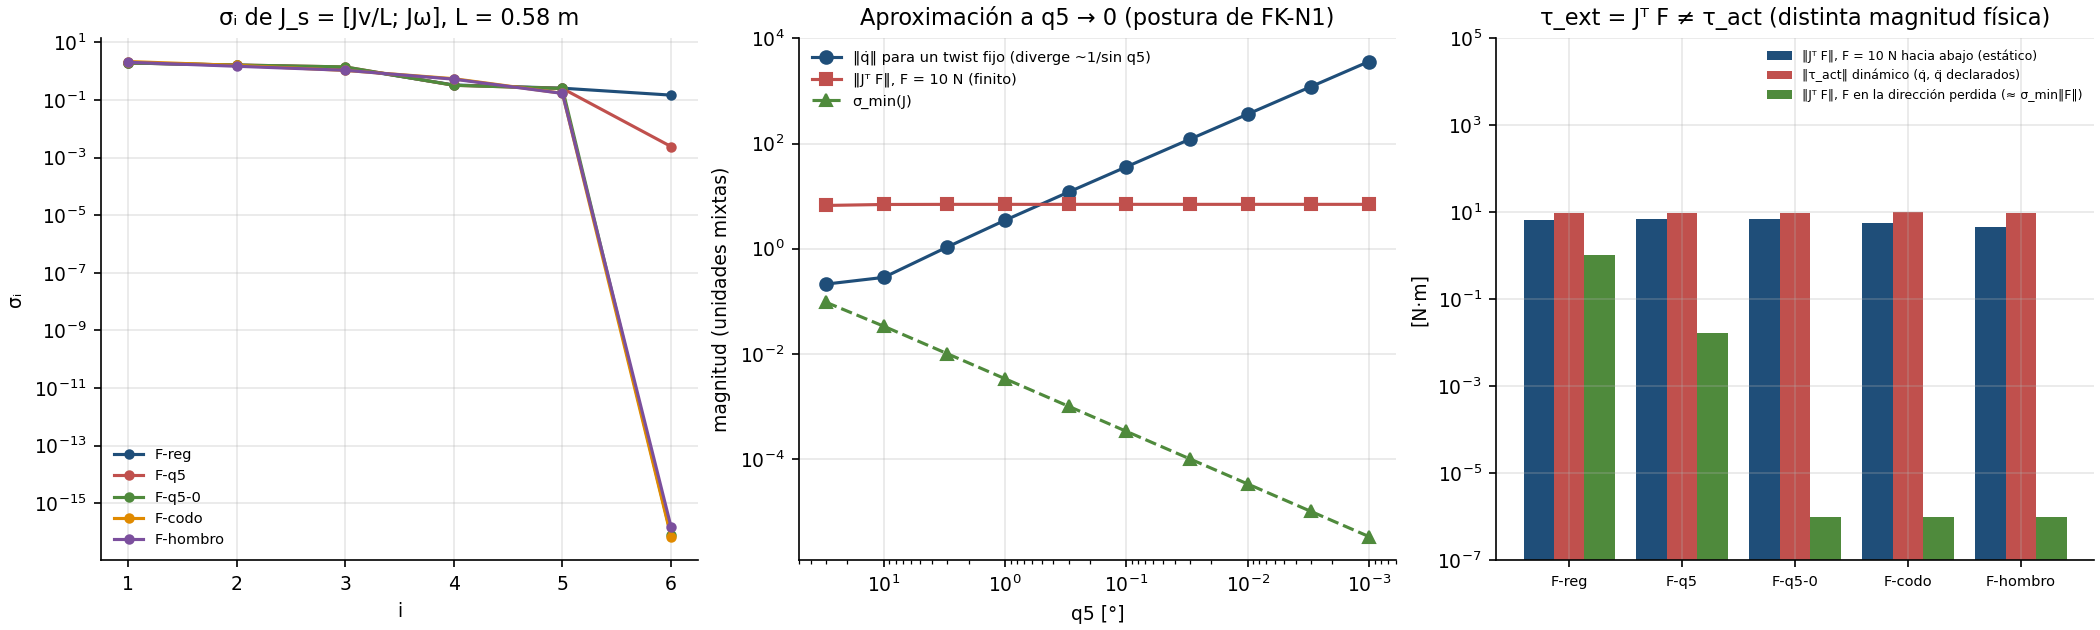
\includegraphics[width=0.9\textwidth]{../resultados/figuras/singularidad_svd_tau.png}
\caption{Valores singulares de $J_s$ frente al umbral $\tau_{num}$ en los casos de la tabla P4.}
\end{figure}

Los casos F-reg, F-q5, F-q5-0, F-codo, F-hombro y F-TAU quedan \textit{verificados} (S0, análisis algebraico del modelo, sin datos físicos). Ninguno corresponde a una medición en el robot. Los valores de $\tau_{act}$ son del modelo dinámico propio (\texttt{dynamics.py}); no se midieron torques ni corrientes.

% ---------------------------------------------------------------- 8
\section{Sincronización, tolerancias y presupuesto (Bloques G y H)}
\label{sec:tol}

\textbf{Todo lo de esta sección está pendiente de aprobación docente.} El documento oficial presenta los umbrales como propuesta y la rúbrica exige no presumir cifras aprobadas.

\textbf{Sincronización (G).} La FK evaluada en $\mathbf{q}(t_1)$ solo es comparable con la pose de $t_2$ si hay estado estático o alineación temporal. En FK-N1 y FK-N2 la adquisición es secuencial (lectura de $\mathbf{q}$, pose y de nuevo $\mathbf{q}$); se aceptan las muestras con $\Delta q\le10^{-3}\,^\circ$ y ventana $\le500$~ms. La ventana observada tiene mediana 14,2 y 15,0~ms y máximo 54,3 y 33,7~ms (N1 y N2). No hay reloj común con el controlador. Sin robot estacionario el caso se clasificaría \textit{inconcluso por tiempo}.

\textbf{Presupuesto offline (G).} Para FK propia frente a la referencia en doble precisión, $\tau_p=K\epsilon_{mach}L\,N_{ops}$ y $\tau_R=K\epsilon_{mach}N_{ops}$, con $N_{ops}=700$, $L=0{,}942$~m y $K$ declarado.

% Generado por hito3.validacion; requiere \usepackage{booktabs,array}
\begin{table}[htbp]
\centering
\scriptsize
\setlength{\tabcolsep}{3pt}
\renewcommand{\arraystretch}{1.15}
\caption{Presupuesto numérico offline ($\epsilon=2.220e-16$, $N_{ops}=700$, $L=0.942$ m; $K=10$ declarado). Error máximo observado FK propia vs ROS-Industrial: $e_p=2.49e-16$ m, $e_R=8.10e-16$ rad (atan2). Estado: pendiente de aprobación.}
\label{tab:G}
\begin{tabular}{lrr}
\toprule
\textbf{$K$} & \textbf{$\tau_p=K\epsilon L N_{ops}$ [m]} & \textbf{$\tau_R=K\epsilon N_{ops}$ [rad]} \\
\midrule
$1$ & $1.46\times10^{-13}$ & $1.55\times10^{-13}$ \\
$4$ & $5.86\times10^{-13}$ & $6.22\times10^{-13}$ \\
$10$ & $1.46\times10^{-12}$ & $1.55\times10^{-12}$ \\
$1e+02$ & $1.46\times10^{-11}$ & $1.55\times10^{-11}$ \\
\bottomrule
\end{tabular}
\end{table}


$K$ y $N_{ops}$ son estimaciones del equipo. El error máximo observado (\SI{2,49e-16}{m} y \SI{8,10e-16}{rad}) queda varios órdenes por debajo de cualquier fila; no se ha fijado ninguna fila como umbral. Para el cribado sintético el documento oficial propone $10^{-6}$~m y $10^{-5}$~rad. Estos valores son \textit{pendientes de aprobación}; no son tolerancias físicas ni valores de ABB.

\textbf{Incertidumbres frente al IRC5 (H).} No se fija ninguna cifra de tolerancia frente al controlador: la tabla siguiente enumera las fuentes de incertidumbre y su estado. El criterio estricto de $10^{-6}$ m y $10^{-6}$ rad del proyecto es una decisión del equipo, no un requisito oficial.

% Generado por hito3.validacion; requiere \usepackage{booktabs,longtable,array}
\begingroup
\scriptsize
\setlength{\tabcolsep}{2.5pt}
\renewcommand{\arraystretch}{1.12}
\begin{longtable}{p{3.6cm}p{6.2cm}p{3cm}p{2.6cm}}
\caption{Incertidumbres de la comparación FK propia vs IRC5. No existe umbral numérico aprobado: estado pendiente y bloqueado por datos.}\label{tab:H}\\
\toprule
\textbf{Fuente de incertidumbre} & \textbf{Valor / cota} & \textbf{Origen} & \textbf{Estado} \\
\midrule
\endfirsthead
\toprule
\textbf{Fuente de incertidumbre} & \textbf{Valor / cota} & \textbf{Origen} & \textbf{Estado} \\
\midrule
\endhead
\bottomrule
\endfoot
Resoluci\'on de la posici\'on del robtarget (xyz) & 7 cifras significativas: 4 decimales en mm (1e-4 mm = 1e-7 m) si |v| $\ge$ 100 mm; hasta 6 decimales si |v| < 10 mm & observado en los registros S1 (FK-N1; cota de FK-N2: 7.1e-08 m) & cota derivada; umbral pendiente \\
Resoluci\'on del cuaterni\'on (w,x,y,z) & $\le$ 7 cifras significativas observadas (componentes $\le$ 1) & observado; cota 2$\cdot$||$\delta$q||, |$\delta$q\_i| $\le$ 5e-8 & cota derivada; umbral pendiente \\
Resoluci\'on de q (RWS entrega float32) & semi-ulp float32 hasta 7.6e-06 $^\circ$ en FK-N1 & derivado: $\Sigma$$\Vert$Jv\_i$\Vert$$\cdot$semi-ulp (FK-N1) & cota derivada; umbral pendiente \\
Cota total de cuantizaci\'on de los datos (FK-N1 / FK-N2) & e\_p $\le$ 1.18e-07 / 7.78e-08 m; e\_R $\le$ 5.00e-07 / 4.13e-07 rad & suma de las tres fuentes anteriores & piso de resoluci\'on, no tolerancia \\
TCP / herramienta activa & tooldata del IRC5 NO le\'ido; se compara tool0 (brida) $\Rightarrow$ TCP no interviene; TCP de 0.150 m es convenci\'on del modelo (tcp\_verified\_on\_robot: false) & no medido & bloqueado por datos \\
Sincron\'ia q $\leftrightarrow$ pose & ventana q$\to$pose$\to$q: mediana 14.2 / 15.0 ms, m\'ax 54.3 / 33.7 ms (N1/N2); sin reloj com\'un, robot estacionario & observado (window\_ms) & mitigada con q\_antes $\approx$ q\_despu\'es; no medible por debajo de la ventana \\
Fluctuaci\'on de la pose del IRC5 con q constante & hasta e\_p = 2.44e-06 m y e\_R = 1.32e-05 rad en las 155 muestras FUERA & observado (diagn\'ostico FUERA) & causa indeterminada por datos \\
Base y ceros mec\'anicos del controlador frente al modelo & coincidencia emp\'irica en 2 posturas distintas (error $\le$ \textasciitilde{}1e-6 m); calibraci\'on de f\'abrica del robot no consultada & no medido directamente & parcial \\
Repetibilidad / exactitud absoluta del IRB 120 & no medida en este trabajo; el repositorio cita 0.01 mm de repetibilidad (hito2/irb120/validation.py, de la hoja ABB) sin verificaci\'on local & cita no verificada & bloqueada por datos \\
\end{longtable}
\endgroup


Estado: TOL-OFF (\textit{parcial}, presupuesto sin aprobación), TOL-IRC5 (\textit{parcial}: no se inventa ninguna tolerancia física). La repetibilidad del IRB~120 que cita el repositorio (0,01~mm, hoja ABB) no se verificó localmente.

% ---------------------------------------------------------------- 9
\section{Integración y movimiento (Gate 3)}
\label{sec:gate3}

\subsection{Evidencia de movimiento PC$\to$IRC5}
Fuente: \ruta{hito3/docs/evidencia_gate3_movimiento.md} y la tabla por orden \ruta{hito3/docs/gate3_ordenes.csv} (265 filas), extraídas de los \texttt{jsonl} del controlador, que no están versionados. Horas locales UTC$-4$.

\begin{table}[H]
\centering\small
\renewcommand{\arraystretch}{1.15}
\begin{tabular}{@{}llrrrrr@{}}
\toprule
\textbf{Sesión} & \textbf{Fecha (hora local)} & \textbf{Módulo} & \textbf{Órdenes} & \textbf{Llegadas} & \textbf{Error máx.} & \textbf{Mediana}\\
\midrule
S16 & 16/11 (21:23--21:28) & v2 & 24 & 24 & 0,0159$^\circ$ & 0,0015$^\circ$\\
S17 & 17/11 (21:01--22:53) & v2/v3/v4 & 177 & 177 & 0,1862$^\circ$ & 0,0068$^\circ$\\
S18 & 18/11 (19:18--19:48) & v4 & 59 & 58 & 0,0689$^\circ$ & 0,0081$^\circ$\\
S19 & 19/11 (17:27--17:29) & v4 (inferida) & 5 & 5 & 0,0537$^\circ$ & 0,0103$^\circ$\\
\midrule
\textbf{Total} & & & \textbf{265} & \textbf{264} & 0,1862$^\circ$ & \\
\bottomrule
\end{tabular}
\caption{Órdenes de movimiento registradas. Código de resultado 2 = llegada confirmada.}
\end{table}

Eslabón a eslabón del criterio S3 (orden verificable $\to$ aceptación $\to$ estado $\to$ movimiento observado):
\begin{enumerate}[leftmargin=*]
\item \textbf{Orden verificable.} Cada orden tiene la escritura de \texttt{pcTarget} (HTTP 204) y un evento \texttt{order} con \texttt{seq}, \texttt{from\_deg} y \texttt{target\_deg}. La PC sube \texttt{pcSeq} solo después de leer de vuelta \texttt{pcTarget}; el registro no guarda el valor leído de vuelta.
\item \textbf{Aceptación.} \texttt{rbCodigo} final igual a 2 implica que RAPID validó y ejecutó; los rechazos tendrían códigos $-1\dots-5$ y no aparecen. No se registra el instante de aceptación ni el código intermedio 1.
\item \textbf{Estado.} \texttt{joints\_deg} leído por RWS al terminar cada orden. \texttt{opmode} y \texttt{ctrlstate} durante la orden no se guardan.
\item \textbf{Movimiento observado.} Medido por el propio controlador ($q_{llegada}\neq q_{partida}$); la observación humana consta solo en la bitácora. No hay video, foto con hora ni medición externa.
\item \textbf{Autorización GO.} \textbf{No consta} ninguna autorización firmada, nombres ni alcance.
\end{enumerate}

\textbf{Clasificación:} \textbf{S3 técnico con alcance acotado} (movimientos articulares \texttt{MoveAbsJ} dentro de los límites del RAPID, margen de 2$^\circ$, paso máximo de 10$^\circ$ en v2 y de 45$^\circ$ en v3/v4); \textbf{GO sin firmar}, por lo que el Gate~3 formal (S3 autorizado) \textbf{no está acreditado}. Estado P5 de S3-MOV: \textit{parcial}.

Observaciones que no se ocultan:
\begin{itemize}[leftmargin=*]
\item La orden 59 del 18/11 (J1, $\Delta_{\max}=38{,}6^\circ$) no tiene evento de resultado: no se afirma llegada ni rechazo. Por eso son 264 y no 265 llegadas.
\item Huecos de numeración: S17 empieza en la orden 43 y S19 en la 98; no se rellenan.
\item Hubo 2 escrituras de $J5$ con HTTP 403 el 16/11 (tras detener y reanudar RAPID) sin orden resultante; la corrección está en el código y J5 se movió después sin 403, pero el escenario no se repitió a propósito.
\item La primera tanda de S17 tiene errores mayores (15 órdenes entre 0,05$^\circ$ y 0,19$^\circ$); la causa no se investigó.
\item Velocidad: v2 y v3 fijan 20~mm/s y 5$^\circ$/s; v4 usa porcentaje de $[250,60,250,60]$, con órdenes a 12, 17, 50, 65 y 75\,\%. Las velocidades y aceleraciones reales no se midieron.
\item Modo: S16 en manual reducido con habilitador (bitácora); la primera tanda de S17 en manual (\textit{inferido}); el resto en AUTO sin habilitador según la bitácora. La aceptación de ese modo por el laboratorio no consta.
\end{itemize}

\subsection{Panel de RViz}
El panel «IRB 120» de RViz (paquetes \texttt{irb120\_rviz\_panel} e \texttt{irb120\_control}) envía las órdenes de las sesiones S17 a S19 y calcula IK/FK antes de enviar; bloquea el envío si falla la verificación IK$\to$FK, la ida y vuelta o la comparación modelo--controlador. Según \ruta{hito3/docs/niveles_evidencia.md}, con robot simulado pasan las pruebas offline (\texttt{./brazo.sh pruebas}); esas pruebas no se ejecutaron al preparar este informe y no se afirma corrección de la IK/FK del panel fuera de las posturas probadas. El flujo es PC (RViz) $\to$ RWS $\to$ RAPID, no \texttt{ros2\_control} ni EGM.

\subsection{Elementos que son solo S0 (simulación)}
\begin{itemize}[leftmargin=*]
\item \textbf{RAPID v5 y \texttt{MoveL}.} El código existe (4667 caracteres, por debajo del límite de 4900) pero \textbf{no se compiló ni se probó en el IRC5}: no se puede afirmar que su sintaxis sea válida ni que funcionen \texttt{MoveL} o \texttt{ConfL}.
\item \textbf{Planificador de trayectorias A$\to$B$\to$C$\to$A y Estudio (CustomTkinter).} Evalúa tramos articulares y lineales y muestrea $\sigma_{\min}$, $\kappa$, límites, $\dot{\mathbf{q}}$, $\ddot{\mathbf{q}}$ y $\tau$; probado offline y con el panel simulado. Las reglas más estrictas que las del Hito~2 son una decisión del equipo, no un criterio aprobado.
\item \textbf{Celda PLC S7-1200 $\leftrightarrow$ PC $\leftrightarrow$ robot.} Nodos ROS~2 independientes con telegramas de dos palabras (núcleo) y parte extendida, probados con PLC y panel simulados. Sin PLC real; el bloque SCL no se compiló en TIA Portal; ningún movimiento ordenado desde el PLC.
\item \textbf{EGM.} 24 pruebas offline con EGM UDP simulado (\textit{loopback}); sin comunicación EGM con el controlador (\texttt{physical\_motion\_tested: false}).
\end{itemize}

% ---------------------------------------------------------------- 10
\section{Seguridad y reproducibilidad}
\label{sec:seg}

\subsection{Checklist de seguridad}
La plantilla de \ruta{hito3/docs/checklist_seguridad.md} contiene 11 puertas previas al Gate~3. \textbf{Ninguna se marca cumplida}, porque la autoridad que debe confirmarla no ha firmado; todas están en estado \textit{pendiente}. Lo que sí consta: identidad y versión del robot (puerta 1, parcial, falta la placa del controlador), límites articulares y velocidad reducida en RAPID (puerta 8, parcial; el TCP de 0,150~m no está medido y no está definido si 75\,\% cuenta como velocidad reducida), y registro técnico por orden (puerta 10; el protocolo aprobado no consta). Los registros de decisión GO/NO-GO de S16 a S19 están vacíos a propósito para firma del responsable del laboratorio; una firma posterior no convierte en autorizada una sesión pasada.

Estado inicial de toda sesión: NO-GO para movimiento físico. La plantilla incluye una versión de 14 puertas para la próxima sesión, en blanco.

\subsection{Reproducibilidad}
Desde la carpeta \texttt{proyecto/} del repositorio:
\begin{itemize}[leftmargin=*]
\item Validación completa: \texttt{python3 -m hito3.validacion}. Regenera resultados, manifiestos y tablas \LaTeX.
\item Pruebas del paquete: \texttt{python3 -m pytest hito3/tests -q}. Resultado al preparar este informe: 10 pruebas aprobadas.
\item Pruebas offline del resto del proyecto (panel, RWS simulado): \texttt{./brazo.sh pruebas}. Estas \textbf{no se ejecutaron} para este informe.
\item Compilar este informe: \texttt{make -C hito3/informe}.
\end{itemize}
Las entradas reales están conservadas en \ruta{hito3/datos/} (subconjuntos estacionarios, con SHA-256 del archivo crudo y recuento de líneas). Los archivos crudos \texttt{comunicacion\_*.jsonl} (14,1~MB y 16,0~MB) viven en el checkout principal y no están versionados. El código del modelo se identifica por SHA-256 en cada manifiesto. Ejecución anterior consignada: Python 3.14.4, NumPy 2.3.5, SciPy 1.16.3. Una ejecución desde cero en una máquina limpia no se ha realizado.

% ---------------------------------------------------------------- 11
\section{Estados formales P5, checklist P6 y firma P7}
\label{sec:p5p7}

\subsection{P5: estado por caso}
\newgeometry{margin=1.2cm}
\begin{landscape}
% Generado por hito3.validacion; requiere \usepackage{booktabs,longtable,array}
\begingroup
\scriptsize
\setlength{\tabcolsep}{2.5pt}
\renewcommand{\arraystretch}{1.12}
\begin{longtable}{lllp{9cm}}
\caption{P5. Estado formal de decisión y nivel de evidencia por caso. «Verificado» = verificación procedimental (umbrales pendientes de aprobación docente).}\label{tab:P5}\\
\toprule
\textbf{Caso} & \textbf{Nivel} & \textbf{Estado P5} & \textbf{Justificación (resumen)} \\
\midrule
\endfirsthead
\toprule
\textbf{Caso} & \textbf{Nivel} & \textbf{Estado P5} & \textbf{Justificación (resumen)} \\
\midrule
\endhead
\bottomrule
\endfoot
FK-N1 & S1 & parcial & Observaci\'on del controlador por RWS con unidad, fuente y marca temporal (S1). No es S2 (no trazada por ROS) ni S3. Parcial: umbral no aprobado; una so... \\
FK-N1-S0 & S0 & verificado & Modelo vs modelo. rosi\_model es independiente de la TABLA DH y del c\'odigo propio, no de la geometr\'ia nominal ABB: no demuestra exactitud f\'isica. \\
FK-N2 & S1 & parcial & Observaci\'on del controlador por RWS con unidad, fuente y marca temporal (S1). No es S2 (no trazada por ROS) ni S3. Parcial: umbral no aprobado; una so... \\
FK-N2-S0 & S0 & verificado & Modelo vs modelo. rosi\_model es independiente de la TABLA DH y del c\'odigo propio, no de la geometr\'ia nominal ABB: no demuestra exactitud f\'isica. \\
FK-N3 & S1 & parcial & Lectura de pantalla del controlador (S1 limitado): sin tiempo simult\'aneo ni registro autom\'atico; solo apoyo complementario. \\
FK-L & S0 & verificado & Offline contra rosi\_model; los l\'imites son los documentados de la hoja ABB (dh.py), no le\'idos del controlador. \\
FK-L-REAL & S1 (pendiente) & bloqueado por acceso & Depende de permiso/hardware no disponibles. \\
FK-D-TCP & S1 & verificado & Datos reales S1 + perturbaci\'on offline declarada: demuestra la sensibilidad a la herramienta y la regla de no comparar brida con TCP. \\
FK-D-ORD & S1 & verificado & Datos reales S1 con permutaci\'on offline intencional; el error emerge y desaparece al invertir la permutaci\'on. \\
FK-FUERA & S1 & parcial & Clasificadas con el \'arbol del Bloque C; causa ra\'iz indeterminada por datos (falta registro simult\'aneo y repetici\'on controlada). \\
FK-INV & S1 & parcial & Sin datos que comparar; clasificadas por tipo de excepci\'on. \\
FK-TCP-REAL & S1 (pendiente) & bloqueado por acceso & Depende de acceso al controlador. \\
IK-1 & S0 & verificado & IK propia vs FK propia/independiente y DLS independiente; offline. \\
IK-2 & S0 & verificado & IK propia vs FK propia/independiente y DLS independiente; offline. \\
IK-3 & S0 & verificado & IK propia vs FK propia/independiente y DLS independiente; offline. \\
IK-4 & S0 & parcial & IK propia vs FK propia/independiente y DLS independiente; offline. \\
IK-5 & S0 & verificado & IK propia vs FK propia/independiente y DLS independiente; offline. \\
IK-REAL & S3 (no alcanzado) & bloqueado por acceso & NO-GO f\'isico; plan alternativo: IK offline (IK-1..IK-5). \\
S3-MOV & S3 t\'ecnico (registrado); S3 autorizado no acreditado & parcial & Ver hito3/docs/evidencia\_gate3\_movimiento.md y gate3\_ordenes.csv; firmar checklist\_seguridad.md en la pr\'oxima sesi\'on. \\
J-N1 & S0 & verificado & J propio vs diferenciaci\'on num\'erica de la FK independiente; dominado por el error de FD, no por el J. \\
J-N2 & S0 & verificado & J propio vs diferenciaci\'on num\'erica de la FK independiente; dominado por el error de FD, no por el J. \\
J-N3 & S0 & verificado & J propio vs diferenciaci\'on num\'erica de la FK independiente; dominado por el error de FD, no por el J. \\
J-N4 & S0 & verificado & J propio vs diferenciaci\'on num\'erica de la FK independiente; dominado por el error de FD, no por el J. \\
J-FD & S0 & verificado & Caracterizaci\'on num\'erica de la referencia por FD (autoconvergencia). \\
J-REAL & S1/S3 (no alcanzado) & bloqueado por acceso & Depende de hardware y GO. \\
F-reg & S0 & verificado & An\'alisis algebraico del modelo; sin datos f\'isicos. \\
F-q5 & S0 & verificado & An\'alisis algebraico del modelo; sin datos f\'isicos. \\
F-q5-0 & S0 & verificado & An\'alisis algebraico del modelo; sin datos f\'isicos. \\
F-codo & S0 & verificado & An\'alisis algebraico del modelo; sin datos f\'isicos. \\
F-hombro & S0 & verificado & An\'alisis algebraico del modelo; sin datos f\'isicos. \\
F-TAU & S0 & verificado & Demostraci\'on algebraica sobre el modelo propio. \\
MET-SINT & S0 & verificado & Valores esperados del documento. \\
TOL-OFF & S0 & parcial & Presupuesto num\'erico declarado, sin aprobaci\'on; K y N\_ops son estimaciones. \\
TOL-IRC5 & S1 & parcial & No se inventa ninguna tolerancia f\'isica. \\
\end{longtable}
\endgroup

\end{landscape}
\restoregeometry

\subsection{P6: checklist antes de declarar un resultado}
Marcado según \ruta{hito3/docs/checklist_P6_P7.md} (actualizado el 24/11/2026 con los resultados del paquete). \textbf{Cumple}: existe la evidencia indicada. \textbf{Parcial}: existe pero incompleta.

\begin{table}[H]
\centering\scriptsize
\renewcommand{\arraystretch}{1.15}
\begin{tabularx}{\textwidth}{@{}r>{\raggedright\arraybackslash}p{4.6cm}>{\raggedright\arraybackslash}p{1.5cm}>{\raggedright\arraybackslash}X@{}}
\toprule
\textbf{\#} & \textbf{Punto oficial} & \textbf{Estado} & \textbf{Evidencia y brecha}\\
\midrule
1 & $\mathbf{q}$, \texttt{joint\_order}, unidades, signos, offsets y fuente & Parcial & Declarados en los manifiestos; \texttt{controller\_joint\_mapping\_verified: false}; J4--J6 variaron poco.\\
2 & Modelo/URDF/commit, parámetros, tool y TCP & Parcial & SHA-256 y commit en manifiestos; TCP 0,150~m es convención; \texttt{tooldata} sin leer.\\
3 & Base, TCP y tiempo comparables & Parcial & \texttt{tool0}, \texttt{wobj0}, \texttt{Base}, robot estacionario; sin reloj común; sin TCP real.\\
4 & Referencia identificada e independencia & Cumple & IRC5 (independiente del modelo) y \texttt{rosi\_model} (independiente de la tabla DH, no de la geometría nominal); URDF clasificado como no independiente.\\
5 & $\ep$ y $\eR$ en m y rad & Cumple & P1, \ruta{validation_cases.csv}, errores por muestra.\\
6 & IK: ramas, límites y residuo FK por rama & Cumple (S0) & P2, 40 ramas clasificadas.\\
7 & $J$: twist, columna, punto, FD y paso $h$ & Cumple (S0) & P3, curva $h\to E(h)$.\\
8 & Singularidad: tarea, rango/$\sigma_i$ y $L$ & Cumple (S0) & P4, $L=0{,}58$~m, $\tau_{num}$.\\
9 & $J^TF$ distinto de dinámica; sin torque infinito & Cumple (S0) & F-TAU y P4.\\
10 & Presupuesto o criterio de tolerancia y estado de aprobación & Parcial & Presupuesto offline y fuentes de incertidumbre declarados; estado \textit{pendiente de aprobación}; sin umbral aprobado.\\
11 & Script ejecuta offline con entradas conservadas & Parcial & \texttt{python3 -m hito3.validacion} y 10 pruebas aprobadas; entradas en \texttt{hito3/datos}; falta ejecución en máquina limpia.\\
12 & Logs, fecha, responsable y evidencia citados & Parcial & Fechas, rutas y SHA-256 citados; \textbf{responsable por prueba: no consta}.\\
13 & No afirmo movimiento ni GO sin autorización & Cumple & Se separa S3 técnico de S3 autorizado; GO sin firmar.\\
\bottomrule
\end{tabularx}
\caption{Checklist P6. Recuento: 7 cumplen (4 a 9 y 13), 6 parciales (1, 2, 3, 10, 11, 12), 0 no cumplen.}
\end{table}

\subsection{P7: firma de revisión}
\label{sec:p7}
\textbf{Ninguna firma registrada.} La plantilla queda en blanco hasta que el autor y el docente revisen.

\begin{table}[H]
\centering\small
\renewcommand{\arraystretch}{1.5}
\begin{tabularx}{\textwidth}{@{}>{\bfseries}p{4.2cm}X@{}}
\toprule
Equipo & \\
ID de prueba & \\
Responsable & \\
Versión del documento & \\
Fecha & \\
Revisión docente & $\square$ pendiente \quad $\square$ revisado \quad $\square$ aprobado (alcance explícito): \rule{4cm}{0.3pt}\\
Hallazgo mayor & \\
Acción siguiente & \\
Enlace a la evidencia & \\
\bottomrule
\end{tabularx}
\caption{Firma P7 (en blanco).}
\end{table}

% ---------------------------------------------------------------- 12
\section{Limitaciones y trabajo pendiente}
\label{sec:pend}

\subsection{Limitaciones del trabajo actual}
\begin{itemize}[leftmargin=*]
\item La comparación física cubre dos posturas y, en cada una, lecturas repetidas de una sola postura; J4--J6 variaron poco. No es una cobertura del espacio de trabajo.
\item La referencia independiente (ROS-Industrial) comparte la geometría nominal con el modelo propio: valida la implementación, no la exactitud mecánica.
\item Las 155 muestras FUERA y las 6263 lecturas inválidas no tienen causa raíz demostrada.
\item Las tolerancias son propuestas y la repetibilidad citada del IRB~120 no se verificó.
\item La ruta es RWS + RAPID: una orden a la vez, no control continuo; las velocidades reales no se midieron.
\item El estado S3 técnico no es S3 autorizado; los \texttt{jsonl} no están versionados.
\end{itemize}

\subsection{Trabajo pendiente para la próxima sesión de laboratorio}
\begin{enumerate}[leftmargin=*]
\item Obtener el GO/NO-GO firmado por el responsable del laboratorio \textbf{antes} de mover, con alcance exacto y modo permitido (en particular AUTO sin habilitador), y guardar el escaneo.
\item Registrar nombre del operador y responsable, procedimiento local escrito, placa del controlador y revisión.
\item Observación independiente del movimiento: video o foto fechados y anotación de quién está en el FlexPendant.
\item Registrar \texttt{opmode}, \texttt{ctrlstate} y el valor leído de vuelta de \texttt{pcTarget} por orden; copiar los \texttt{jsonl} a una carpeta versionada.
\item Provocar a propósito «detener y reanudar RAPID» para comprobar la corrección del HTTP 403.
\item Leer el \texttt{tooldata} real por RWS y medir el TCP; repetir la comparación FK en el TCP físico.
\item Comparar FK en posturas con J4--J6 variados y repetir la adquisición con registro simultáneo para explicar las muestras FUERA.
\item Probar la v5 en el IRC5 solo con un primer tramo articular corto a 10--20\,\% y con la v4 respaldada.
\item Pedir al docente la aprobación o los umbrales de FK/IK/$J$ y cerrar los estados P5.
\item Asignar responsables por tarea y preparar la defensa individual.
\item Decidir con el docente si EGM es exigible (ruta B).
\end{enumerate}

\end{document}
